\section{VECTƠ TRONG KHÔNG GIAN}
\subsection{LÝ THUYẾT CẦN NHỚ}
\subsubsection{Tổng của hai véc tơ}
\begin{enumerate}[\iconMT]
	\item \indam{Định nghĩa:}
	\immini{Trong không gian, cho hai véctơ $\vec{a}$ và $\vec{b}$. Lấy ba điểm $O$, $A$, $B$ sao cho $\vec{OA}=\vec{a}$, $\vec{AB}=\vec{b}$. Ta gọi $\vec{OB}$ là \indamm{tổng của hai véctơ} $\vec{a}$ và $\vec{b}$, ký hiệu $\vec{a}+\vec{b}$.\\
		Phép lấy tổng của hai véctơ $\vec{a}$ và $\vec{b}$ được gọi là \indamm{phép cộng véctơ}.}
	{ \hspace{1cm}
	\begin{tikzpicture}[>=stealth,scale=.5,font=\footnotesize]
		\foreach \x\y\t in {3/0.4/A1,4./4.4/A2,9.5/4.3/B1,14.5/1.3/B2,5/0/O}
		\coordinate (\t) at (\x,\y);
		\coordinate (A) at ($(A2)-(A1)+(O)$);
		\coordinate (B) at ($(B2)-(B1)+(A)$);
		\foreach \a/\b in {A1/A2,B1/B2,O/A,A/B,O/B}
		{\draw[-{Stealth[length=2.5mm]}](\a)--(\b);}
		\node at ($(A1)!1/2!(A2)$)[left=-2pt]{$\vec{a}$};
		\node at ($(B1)!1/2!(B2)$)[above right=-2pt]{$\vec{b}$};
		\node at ($(O)!1/2!(A)$)[left=-2pt]{$\vec{a}$};
		\node at ($(A)!1/2!(B)$)[above right=-2pt]{$\vec{b}$};
		\node at ($(O)!1/2!(B)$)[rotate=7,above=-2pt]{$\vec{a}+\vec{b}$};
		\foreach \t/\g in {O/-140,A/90,B/0}
		\draw[fill=black] (\t)circle(1.2pt) +(\g:12pt)node{$\t$};
\end{tikzpicture}}
		\item \indam{Các quy tắc cần nhớ:} 
	\begin{listEX}[1]
	\immini{\item [\ding{172}] Quy tắc ba điểm: Với ba điểm $A$, $B$, $C$, ta có
		\boxminit{$\vec{AB}  + \vec{BC}  = \vec{AC}$}
		\item [\ding{173}] Quy tắc hình bình hành: Cho $ABCD$ là hình bình hành, ta có
	\boxminit{$\vec{AB}  + \vec{AD}  = \vec{AC}$}}{
	\begin{tikzpicture}[scale=0.6, font=\footnotesize, line join=round, line cap=round]
		\begin{scope}
			\foreach \x\y\t in {0/0/A, -2/-2/B, 2.5/-1.5/C}
			\coordinate (\t) at (\x,\y);
			\foreach \a\b in {A/B, B/C,A/C}
			\draw[-{Stealth[length=2mm]}] (\a)--(\b);
			\foreach \t\g in {A/90, B/-100, C/-80}
			\draw[fill=black] (\t)circle(0.6pt) +(\g:8pt)node{$\t$};
		\end{scope}
		\begin{scope}[xshift=5cm]
			\foreach \x\y\t in {0/0/A, -1.5/-2/B, 2.5/-2/C,4/0/D}
			\coordinate (\t) at (\x,\y);
			\foreach \a\b in {A/B, A/D,A/C}
			\draw[-{Stealth[length=2mm]}] (\a)--(\b);
			\draw[dashed] (B)--(C)--(D);
			\foreach \t\g in {A/90, B/-90, C/-45,D/50}
			\draw[fill=black] (\t)circle(0.6pt) +(\g:8pt)node{$\t$};
		\end{scope}
\end{tikzpicture}}
		\immini{ \item [\ding{174}] Quy tắc hình hộp:
	Cho hình hộp $ABCD.A'B'C'D'$. Ta có
			\boxminit{$\vec{AB}  + \vec{AD}  + \vec{AA'}  = \vec{AC'}$}
			\begin{luuy}
				Hệ thức tương tự: \quad $\vec{BA}  + \vec{BC}  + \vec{BB'}  = \vec{BD'}$.
			\end{luuy}
		}{
			\begin{tikzpicture}[scale=0.6, font=\footnotesize, line join=round, line cap=round]
				\def\h{4}
				\foreach \x\y\t in {0/0/A',-1/-1.1/B',2.6/-1.1/C'}
				\coordinate (\t) at (\x,\y);
				\coordinate (D') at ($(A')+(C')-(B')$);
				\coordinate (A) at ($(A')+(0,2.5)$);
				\coordinate (B) at ($(B')+(0,2.5)$);
				\coordinate (C) at ($(C')+(0,2.5)$);
				\coordinate (D) at ($(D')+(0,2.5)$);
				\foreach \a\b in {A/B, A/D,A/C}
				\draw[-{Stealth[length=2mm]}] (\a)--(\b);
				\foreach \a\b in {A/A', A/C'}
				\draw[-{Stealth[length=2mm]},dashed] (\a)--(\b);
				\draw (D)--(C)--(B)--(B')--(C')--(D')--(D) (C')--(C);
				\draw[dashed](B')--(A')--(D');
				\foreach \t/\g in {A'/170,B'/-150,C'/-70,D'/0,A/100,B/170,C/-20,D/50}
				\draw[fill=black] (\t) circle(1pt)
				node[shift={(\g:7pt)}]{$\t$};
			\end{tikzpicture}
		} 
	\end{listEX}
	\item \indam{Tính chất:}
	\begin{gachsoc}
		\begin{itemize}
			\item[\ding{172}]Tính chất giao hoán: $\vec{a}+\vec{b}=\vec{b}+\vec{a}$;
			\item[\ding{173}] Tính chất kết hợp: $\left(\vec{a}+\vec{b}\right)+\vec{c}=\vec{a}+\left(\vec{b}+\vec{c}\right)$;
			\item[\ding{174}] Với mọi véctơ $\vec{a}$, ta luôn có: $\vec{a}+\vec{0}=\vec{0}+\vec{a}=\vec{a}$.
			\item[\ding{175}] Tổng của ba véctơ $\vec{a}$, $\vec{b}$, $\vec{c}$:\quad $\vec{a}+\vec{b}+\vec{c}=\left(\vec{a}+\vec{b}\right)+\vec{c}.$
		\end{itemize}
	\end{gachsoc}
\end{enumerate}
\subsubsection{Hiệu của hai véc tơ}
\begin{enumerate}[\iconMT]
	\item \indam{Véctơ đối:}
	\begin{listEX}[1]
		\item [\ding{172}] Vectơ đối của $\vec{a}$ kí hiệu là $-\vec{a}$.
		\item [\ding{173}] Vectơ đối của $\vec{AB}$ là $\vec{BA}$, nghĩa là $-\vec{AB}=\vec{BA}$ (\textit{dùng để làm mất dấu trừ trước vectơ}).
		\item [\ding{174}] Vectơ $\vec{0}$ được coi là vectơ đối của chính nó.
	\end{listEX}
\vspace{-0.7cm}
\immini{
	\item \indam{Định nghĩa hiệu của hai véctơ:} Trong không gian, cho hai véctơ $\vec{a}$, $\vec{b}$. Ta gọi $\vec{a}+\left(-\vec{b}\right)$ là \indamm{hiệu của hai véctơ} $\vec{a}$ và $\vec{b}$, ký hiệu $\vec{a}-\vec{b}$.\\
	Phép lấy hiệu của hai véctơ được gọi là \indamm{phép trừ véctơ}.
	\item \indam{ Các quy tắc cần nhớ:}\\
	\begin{tcolorbox}[colframe=cyan,colback=red!3!white,boxrule=0.3mm]
		\begin{listEX}[1]
			\item [\ding{172}] Với ba điểm $A$, $B$, $C$ ta có $\vec{AB}-\vec{AC}=\vec{CB}$.
			\item [\ding{173}] Hai véc tơ $\vec{a}$ và $\vec{b}$ đối nhau thì $\vec{a}+\vec{b}=\vec{0}$.
		\end{listEX}
	\end{tcolorbox}
}{\vspace{0.9cm}\hspace{1cm} 
\begin{tikzpicture}[scale=1, font=\footnotesize, line join=round, line cap=round]
	\foreach \x\y\t in {0/0/O,1.5/1/A,3.1/-0.4/B,-0.3/1/a1,1.1/1.6/b1}
	\coordinate (\t) at (\x,\y);
	\coordinate (a2) at ($(a1)+(A)$);
	\coordinate (b2) at ($(b1)+(B)$);
	\foreach \a\b in {a1/a2, b1/b2,O/A,O/B,B/A}
	\draw[-{Stealth[length=2mm]}] (\a)--(\b);
	\path (a1)--(a2)node[pos=0.5,above left]{$\vec{a}$}
	(b1)--(b2)node[pos=0.5,above]{$\vec{b}$}
	(O)--(A)node[pos=0.5,above left]{$\vec{a}$}
	(O)--(B)node[pos=0.5,below]{$\vec{b}$}
	(B)--(A)node[pos=0.7,right=3pt]{$\vec{a}-\vec{b}$};
	\foreach \t\g in {A/90, O/180, B/0}
	\draw[fill=black] (\t)circle(0.2pt) +(\g:5pt)node{$\t$};
\end{tikzpicture}}
\end{enumerate}
\subsubsection{Tích của một số với một véc-tơ}
\begin{enumerate}[\iconMT]
	\item \indam{Định nghĩa:} Cho số thực $k\ne 0$ và vectơ $\vec{a} \ne \vec{0}$. Tích của một số $k$ với vectơ $\vec{a}$ là một vectơ, kí hiệu là $k\vec{a}$, được xác định như sau:
	\begin{itemize}
		\item Cùng hướng với vectơ $\vec{a}$ nếu $k>0$, ngược hướng với vectơ $\vec{a}$ nếu $k<0$.
		\item Có độ dài bằng $|k| \cdot |\vec{a}|$.
	\end{itemize}
	\begin{luuy}
	$0\cdot \vec{a}=\vec{0}$ và $k\cdot \vec{0}=\vec{0}$.
	\end{luuy}
\immini{\indamm{ Ví dụ:} Theo hình vẽ bên, thì $\vec{b}=3\vec{a}$; $\vec{c}=-2\vec{a}$; $\vec{c}=-\dfrac{2}{3}\vec{b}$.
}{
	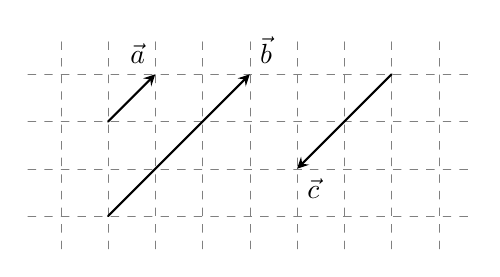
\begin{tikzpicture}[>=stealth,scale=0.6, line join=round, line cap=round]
		\draw[line width=0.05pt,gray,dashed] (-0.7,-0.7) grid (8.7,3.7);
		\draw[->,thick](1,2)--(2,3)node[above left]{$\vec{a}$};
		\draw[->,thick](1,0)--(4,3)node[above right]{$\vec{b}$};
		\draw[->,thick](7,3)--(5,1)node[below right]{$\vec{c}$};
\end{tikzpicture}}
	\item \indam{Hệ thức trung điểm, trọng tâm:}
	\immini{
	\begin{itemize}
		\item [\ding{172}] $I$ là trung điểm của đoạn thẳng $AB$ thì
		\begin{itemize}
			\item [$\bullet$] $\vec{IA}  + \vec{IB}  = \vec 0$;
			\item [$\bullet$] $\vec{IA}=-\vec{IB}$; $\vec{AI}=\dfrac{1}{2}\vec{AB}$;...
		\end{itemize}
		\item [\ding{173}] $G$ là trọng tâm của tam giác $ABC$ thì
		\begin{listEX}[1]
			\item [$\bullet$] $\vec{GA}+\vec{GB}+\vec{GC}=\vec{0}$;
			\item [$\bullet$] $\vec{GA}=-\dfrac{2}{3}\vec{AK}$; $\vec{GA}=-2\vec{GK}$;...
		\end{listEX}
\end{itemize}}{
	\begin{tikzpicture}[scale=0.8, font=\footnotesize, line join=round, line cap=round,thick]
		\begin{scope}
			\foreach \x\y\t in {-2/-2/A, 0/0/B}
			\coordinate (\t) at (\x,\y);
			\coordinate (I) at ($(A)!0.5!(B)$);
			\foreach \a\b in {A/B}
			\draw[] (\a)--(\b);
			\foreach \t\g in {A/-90, B/40,I/1200}
			\draw[fill=black] (\t)circle(0.6pt) +(\g:8pt)node{$\t$};
		\end{scope}
		\begin{scope}[xshift=4cm]
			\foreach \x\y\t in {0/0/A, -2/-2/B, 2.5/-2/C}
			\coordinate (\t) at (\x,\y);
			\coordinate (M) at ($(A)!0.5!(B)$);
			\coordinate (N) at ($(A)!0.5!(C)$);
			\coordinate (K) at ($(C)!0.5!(B)$);
			\coordinate (G) at ($(A)!2/3!(K)$);
			\foreach \a\b in {A/B, B/C, A/C, A/K, M/C, B/N}
			\draw[] (\a)--(\b);
			\foreach \t\g in {A/90, B/-100, C/-80, M/120, N/40, K/-90,G/60}
			\draw[fill=black] (\t)circle(0.8pt) +(\g:10pt)node{$\t$};
		\end{scope}
\end{tikzpicture}}
	\item \indam{Nhận xét:}
	\begin{itemize}
		\item[\ding{172}] Với hai véctơ $\vec{a}$ và $\vec{b}$ bất kỳ, với mọi số $h$ và $k$, ta luôn có
		\begin{gachsoc}
		\begin{enumEX}[$\bullet$]{2}
			\item $k\left(\vec{a}+\vec{b}\right)=k\vec{a}+k\vec{b}$;
			\item $\left(h+k\right)\vec{a}=h\vec{a}+k\vec{a}$;
			\item $h\left(k\vec{a}\right)=\left(hk\right)\vec{a}$;
			\item $1\cdot \vec{a}=\vec{a}$;
			\item $\left(-1\right)\cdot\vec{a}=-\vec{a}$;
			\item $k\vec{a}=\vec{0} \Leftrightarrow \hoac{&\vec{a}=\vec{0}\\& k=0}$.
		\end{enumEX}
	\end{gachsoc}
		\item[\ding{173}] Hai véctơ $\vec{a}$ và $\vec{b}$ ($\vec{b}$ khác $\vec{0}$) cùng phương khi và chỉ khi có số $k$ sao cho $\vec{a}=k\vec{b}$.
		\item[\ding{174}] Ba điểm phân biệt $A$, $B$, $C$ thẳng hàng khi và chỉ khi có số $k \neq 0$ để $\vec{AB}=k\vec{AC}$.
	\end{itemize}
\end{enumerate}
\subsubsection{Tích vô hướng của hai véc-tơ}
\begin{enumerate}[\iconMT]
	\item \indam{Góc giữa hai véctơ:}
	\immini{
			Trong không gian, cho $\vec{u}$ và $\vec{v}$ là hai véctơ khác $\vec{0}$. Lấy một điểm $A$ bất kỳ, gọi $B$ và $C$ là hai điểm sao cho $\vec{AB}=\vec{u}$, $\vec{AC}=\vec{v}$. Khi đó, ta gọi $\widehat{BAC}$ là góc giữa hai véctơ $\vec{u}$ và $\vec{v}$, ký hiệu $\left(\vec{u}, \vec{v}\right)$.
			\begin{luuy}
				$0^{\circ} \leq \left(\vec{u},\vec{v}\right) \leq 180^{\circ}$.
			\end{luuy}
			\begin{gachsoc}
				\begin{itemize}
					\item [$\bullet$] Nếu $\vec{u}$ cùng hướng với $\vec{v}$ thì $\left(\vec{u}, \vec{v}\right)=0^\circ$;
					\item [$\bullet$] Nếu $\vec{u}$ ngược hướng với $\vec{v}$ thì $\left(\vec{u}, \vec{v}\right)=180^\circ$;
					\item [$\bullet$] Nếu $\vec{u}$ vuông góc với $\vec{v}$ thì $\left(\vec{u}, \vec{v}\right)=90^\circ$.
				\end{itemize}
			\end{gachsoc}
}{\vspace{-0.5cm}
		\begin{tikzpicture}[scale=0.8, font=\footnotesize, line join=round, line cap=round]
			\foreach \x\y\t in {0/0/A,2/0.8/B,3.2/-1./C,-1/1/u1,-0.5/-1.5/v1}
			\coordinate (\t) at (\x,\y);
			\coordinate (u2) at ($(u1)+(B)$);
			\coordinate (v2) at ($(v1)+(C)$);
			\draw (-1.5,-1.2)--(3.5,-1.2)--(4.5,1)--(-0.5,1)--cycle;
			\draw[dashed] (A)--(u1) (B)--(u2) (A)--(v1) (C)--(v2);
			\foreach \a\b in {A/B, A/C,u1/u2,v1/v2}
			\draw[-{Stealth[length=2mm]}] (\a)--(\b);
			\foreach \t\g in {A/-170, B/0, C/50}
			\draw[fill=black] (\t)circle(0.6pt) +(\g:8pt)node{$\t$};
			\path (A) pic[draw,angle radius=9]{angle=C--A--B};
			\path 
			(u1)--(u2)node[pos=0.5,above]{$\vec{u}$}
			(v1)--(v2)node[pos=0.5,above]{$\vec{v}$};
	\end{tikzpicture}}
	\item \indam{Định nghĩa tích vô hướng của hai véc tơ:}
	Trong không gian, cho hai véctơ $\vec{u}$ và $\vec{v}$ khác $\vec{0}$. Tích vô hướng của hai véctơ $\vec{u}$ và $\vec{v}$ là một số, kí hiệu $\vec{u} \cdot \vec{v}$, được xác định bởi công thức
	\boxminit{$\vec{u} \cdot \vec{v}=|\vec{u}| \cdot |\vec{v}| \cdot \cos (\vec{u}, \vec{v})$}
	\vspace{-0.6cm}
	\begin{note}
		\begin{itemize}
			\item[\ding{172}] Trong trường hợp $\vec{u}=\vec{0}$ hoặc $\vec{v}=\vec{0}$, ta quy ước $\vec{u} \cdot \vec{v}=0$.
			\item[\ding{173}]  $\vec{u} \cdot \vec{u}=\vec{u}^2=|\vec{u}|^2$; \quad $\vec{u}^2 \geqslant 0$; \quad $ \vec{u}^2 = 0 \Leftrightarrow \vec{u}=\vec{0}$.
			\item[\ding{174}]  Với hai véctơ $\vec{u}$, $\vec{v}$ khác $\vec{0}$, ta có $\cos (\vec{u},\vec{v}) = \dfrac{\vec{u} \cdot \vec{v}}{|\vec{u}| \cdot |\vec{v}|}$
			\item[\ding{175}]  Với hai véctơ $\vec{u}$, $\vec{v}$ khác $\vec{0}$, ta có $\vec{u} \perp \vec{v}  \Leftrightarrow \vec{u} \cdot \vec{v}= 0$.
		\end{itemize}
	\end{note}
	\item \indam{TÍnh chất:} Với ba véctơ $\vec{a}$, $\vec{b}$, $\vec{c}$ và số thực $k$, ta có:
	\begin{enumEX}[$\bullet$]{1}
		\item $\vec{a}  \cdot \vec{b}= \vec{b} \cdot \vec{a}$;
		\item $\vec{a} \cdot \left( {\vec{b} + \vec{c}} \right) = \vec{a}  \cdot \vec{b} + \vec{a} \cdot \vec{c}$;
		\item $(k\vec{a}) \cdot \vec{b}= k(\vec{a}  \cdot \vec{b}) = \vec{a} \cdot (k\vec{b})$.
	\end{enumEX}
\end{enumerate}

\subsection{PHÂN LOẠI VÀ PHƯƠNG PHÁP GIẢI TOÁN}
\begin{dang}{Xác định véc-tơ, chứng minh đẳng thức véc tơ,độ dài véc tơ}
	\begin{enumerate}[\iconCH]
		\item Chú ý các quy tắc như: ba điểm, quy tắc hình bình hành, quy tắc hình hộp...;
		\item Độ dài véc tơ $\vec{AB}$ là độ dài đoạn $AB$;
		\item Độ dài đường cao trong tam giác đều $= \text{cạnh} \times \dfrac{\sqrt{3}}{2}$; Độ dài đường chéo hình vuông $= \text{cạnh} \times \sqrt{2}$; Độ dài đường chéo hình lập phương $= \text{cạnh} \times \sqrt{3}$.
	\end{enumerate}
\end{dang}
\boxmini{BÀI TẬP TỰ LUẬN}
\setcounter{vd}{0}
\begin{vd}
\immini{Cho hình hộp $ABCD.A'B'C'D'$. Hãy xác định các véc-tơ (khác $\vec{0}$) có điểm đầu, điểm cuối là các đỉnh của hình hộp $ABCD.A'B'C'D'$ thỏa
		\begin{tasks}(2)
			\task cùng phương với $\vec{AB}$;
			\task cùng phương $\vec{AA'}$;
			\task bằng với $\vec{AD}$;
			\task bằng với $\vec{A'B}$;
			\task đối với $\vec{CD'}$;
			\task đối với $\vec{B'C}$.
	\end{tasks}}{
\begin{tikzpicture}[scale=0.7, font=\footnotesize,>=stealth]
	%Gán số liệu.
	\def\canhAD{3};\def\canhBA{2};\def\gocBAD{-130};\def\h{3};\def\xdinhA'{-0.5};
	%Gán tọa độ.
	\coordinate (A) at (0,0);
	\coordinate (B) at ($(A)+(\gocBAD:\canhBA)$);
	\coordinate (C) at ($(B)+(0:\canhAD)$);
	\coordinate (D) at ($(A)+(0:\canhAD)$);
	\coordinate (A') at ($(A)+(\xdinhA',\h)$);
	\coordinate (B') at ($(B)+(\xdinhA',\h)$);
	\coordinate (C') at ($(C)+(\xdinhA',\h)$);
	\coordinate (D') at ($(D)+(\xdinhA',\h)$);
	%Vẽ khối lẳng trụ ABCD.A'B'C'D'.
	\draw (A')--(B')--(B)--(C)--(C')--(D')--cycle (B')--(C') (D')--(D)--(C);
	\draw[dashed] (A)--(D) ;
	\draw[->,dashed] (A)--(C');
	\draw[->,dashed] (A)--(A');
	\draw[->, dashed] (A)--(D);
	\draw[->, dashed] (A)--(B);
	\draw[->, dashed] (A)--(C);
	%Gán nhãn.
	\foreach \x/\y in {A/180, B/180, C/0, D/0, A'/180, B'/180, C'/0, D'/0}{\fill (\x) circle(1pt) ($(\x)+(\y:0.3cm)$) node{$\x$};}
\end{tikzpicture}}
	\loigiai{}
\end{vd}
\dongcham{1}
\begin{vd}
	Cho hình chóp $S . A B C D$ có đáy $A B C D$ là hình bình hành. Gọi $M$, $N$, $O$ lần lượt là trung điểm của $A B, C D$ và $AC$. Chứng minh rằng
	\begin{listEX}[2]
		\item $\vec{DA}+\vec{BD}=\vec{MA}+\vec{ND}$;
		\item $\vec{SA}+\vec{SC}=\vec{SB}+\vec{SD}$;
		\item $\vec{SA}+\vec{SB}+\vec{SC}+\vec{SD}=4\vec{SO}$;
		\item $\vec{S D}-\vec{B N}-\vec{C M}=\vec{S C}$.
	\end{listEX}
	\loigiai{
		\immini{\vspace*{-3mm}
			\begin{enumerate}
				\item 
				\item Ta có $\vec{SA}+\vec{SC}=2\vec{SO}$; $\vec{SB}+\vec{SD}=2\vec{SO}$. Suy ra $\vec{SA}+\vec{SC}=\vec{SB}+\vec{SD}$.
				\item Ta có $\vec{SA}+\vec{SC}=2\vec{SO}$; $\vec{SB}+\vec{SD}=2\vec{SO}$. Suy ra
				$$\vec{SA}+\vec{SB}+\vec{SC}+\vec{SD}=4\vec{SO}.$$
				\item Từ câu a, ta có $\vec{BN}=-\vec{DM}$.\\
				Suy ra $\vec{S D}-\vec{B N}-\vec{C M}=\vec{S D}+\vec{DM}-\vec{CM}=\vec{SM}+\vec{MC}=\vec{S C}$.
			\end{enumerate}
		}{
			\begin{tikzpicture}[line join=round, line cap = round, >=stealth, scale=.9,font=\footnotesize]
				\def\a{4}
				\path 	(0:0) coordinate (A)
				++(0:\a) coordinate (D)
				++(-130:\a/2) coordinate (C)
				($(A)+(C)-(D)$) coordinate (B)
				($(A)+(80:0.7*\a)$) coordinate (S)
				(intersection of A--C and B--D) coordinate (O)
				($(A)!0.5!(B)$) coordinate (M)
				($(C)!0.5!(D)$) coordinate (N)
				($(A)!0.5!(C)$) coordinate (O)
				;%giao điểm O
				\draw[dashed] 	(B)--(A)--(D)	(A)--(S) (A)--(C) (B)--(D);
				\draw 	(B)-- (C)--(D)
				(B)--(S)	(C)--(S)	(D)--(S);
				\foreach \x/\g in {A/135,B/-135,C/-45,D/45,S/90,M/-50,N/-30,O/-90}
				\fill[black] 	(\x) circle (1pt)
				($(\g:3mm)+(\x)$) node {$\x$};
				\draw [dashed] (D)--(M) (B)--(N);	
		\end{tikzpicture}}
	}
\end{vd}
\dongcham{12}
\begin{vd}
	Cho hình lập phương  $A B C D . A' B' C' D'$ cạnh bằng $a$. Chứng minh:
	\begin{tasks}(2)
		\task  $\vec{C C'}+\vec{B A}+\vec{D' A'}=\vec{C A'}$.
		\task $\vec{B C}+\vec{D C}+\vec{A A'}=\vec{A C'}$.
		\task $\vec{B'B} + \vec{AD} + \vec{CD} = \vec{B'D}$.
		\task $\vec{BB'} - \vec{C'B'} - \vec{D'C'} = \vec{BD'}$.
		\task $\bigg|\vec{AB}+\vec{A'D'}\bigg|=a\sqrt{2}$.
		\task $\bigg|\vec{AB}+\vec{A'D'}+\vec{AA'}\bigg|=a\sqrt{3}$.
	\end{tasks}
	\loigiai{
			\begin{enumerate}[a)]
			\immini{
				\item Vì $A B C D . A' B' C' D'$ là hình hộp nên $\vec{B A}=\vec{C D}$ và $\vec{D' A'}=\vec{C B}$.\\
				Suy ra $\vec{C C'}+\vec{B A}+\vec{D' A'}=\vec{C C'}+\vec{C D}+\vec{C B}=\vec{C A'}$.
				\item Vì tứ giác $A B C D$ là hình bình hành nên $\vec{B C}=\vec{A D}$ và $\vec{D C}=\vec{A B}$. Áp dụng quy tắc hình hộp suy ra $$\vec{B C}+\vec{D C}+\vec{A A'}=\vec{A D}+\vec{A B}+\vec{A A'}=\vec{A C'}$$
				\item Ta có $\vec{AD} = \vec{B'C'}$, $\vec{CD} = \vec{B'A'}$. Do đó 
				$$\vec{B'B} + \vec{AD} + \vec{CD} = \vec{B'B} + \vec{B'C'} + \vec{B'A'} = \vec{B'D}.$$
				\item Ta có \begin{eqnarray*}
					\vec{BB'} - \vec{C'B'} - \vec{D'C'} &=& \vec{BB'} - \left( \vec{D'C'} + \vec{C'B'} \right) 
					= \vec{BB'} - \vec{D'B'} \\
					&=& \vec{BB'} + \left( - \vec{D'B'}\right)
					= \vec{BB'} + \vec{B'D'}= \vec{BD'}.
				\end{eqnarray*}
			}{
	
			\begin{tikzpicture}[scale=0.8, font=\footnotesize, line join=round, line cap=round]
				\def\h{4}
				\foreach \x\y\t in {0/0/A,-1/-1.1/B,2.6/-1.1/C}
				\coordinate (\t) at (\x,\y);
				\coordinate (D) at ($(A)+(C)-(B)$);
				\coordinate (A') at ($(A)+(0,3.2)$);
				\coordinate (B') at ($(B)+(0,3.2)$);
				\coordinate (C') at ($(C)+(0,3.2)$);
				\coordinate (D') at ($(D)+(0,3.2)$);
				\draw (B')--(A')--(D')--(C')--(B')--(B)--(C)--(D)--(D') (C')--(C);
				\draw[dashed](B)--(A)--(D) (A)--(A');
				\foreach \t/\g in {A/170,B/-150,C/-70,D/0,A'/100,B'/170,C'/-20,D'/50}
				\draw[fill=black] (\t) circle(1pt)
				node[shift={(\g:7pt)}]{$\t$};
			\end{tikzpicture}
		}
			\item Ta có $\big|\vec{AB}+\vec{A'D'}\big|=\big|\vec{AB}+\vec{AD}\big|=\big|\vec{AC}\big|=a\sqrt{2}$.
		\item Ta có $\vec{u}= \vec{AB}+\vec{A'D'}+\vec{AA'}=\vec{AB}+\vec{AD}+\vec{AA'}=\vec{AC'}$. Suy ra
			$\big|\vec{u}\big|=AC'=a\sqrt{3}.$
			\end{enumerate}
			
	}
\end{vd}
\dongcham{34}
\begin{vd}%[2H2H1-4]
	\immini{
		Ba lực $\vec{F_1}$, $\vec{F_2}$, $\vec{F_3}$ cùng tác động vào một vật có phương đôi một vuông góc nhau và có độ lớn lần lượt là $2 \mathrm{\,N}$, $3 \mathrm{\,N}$, $4 \mathrm{\,N}$. 
		\begin{tasks}
			\task Tính độ lớn hợp lực của $\vec{F_2}$, $\vec{F_3}$.
			\task Tính độ lớn hợp lực của ba lực đã cho.
		\end{tasks}}
	{
		\begin{tikzpicture}[scale=1.3, font=\footnotesize, line join=round, line cap=round]
			\foreach \x\y\t in {0/0/O,0/1/a,1.3/0/b,-1.2/-1/c}
			\coordinate (\t) at (\x,\y);
			\foreach \a\b in {O/a,O/b,O/c}
			\draw[-{Stealth[length=2mm]}] (\a)--(\b);
			\path (O)--(a) node[pos=0.5,left]{$\vec{F_1}$}
			(O)--(b) node[pos=0.5,above]{$\vec{F_2}$}
			(O)--(c) node[pos=0.5,above left]{$\vec{F_3}$};
			\path 
			pic[draw,angle radius=4]{right angle=a--O--b}
			pic[draw,angle radius=4]{right angle=c--O--b}
			pic[draw,angle radius=4]{right angle=c--O--a};
	\end{tikzpicture}}
	\loigiai{
		\immini{
			\begin{enumerate}[a)]
				\item Gọi $O$ là vị trí trên vật mà ba lực cùng tác động vào. Gọi$A$, $B$, $C$ là các điểm sao cho $\vec{F_1}=\vec{OA}$, $\vec{F_2}=\vec{OB}$, $\vec{F_3}=\vec{OC}$. Khi đó
				$$\left|\vec{F_2}+\vec{F_3}\right|=OE=\sqrt{3^2+4^2}=5 \text{ N}.$$
				\item Dựng các hình chữ nhật $OBEC$ và $OEFA$ thì ta có
				$$\heva{&\vec{OB}+\vec{OC}=\vec{OE}\\&\vec{OA}+\vec{OE}=\vec{OF}.}$$
				Do đó $\vec{F_1}+\vec{F_2}+\vec{F_3}=\vec{OA}+\vec{OB}+\vec{OC}=\vec{OA}+\vec{OE}=\vec{OF}.$\\
				Vậy độ lớn hợp lực của $F_1$, $\vec{F_2}$ và $\vec{F_3}$ là
				$$\begin{aligned}
					\left|\vec{F_1}+\vec{F_2}+\vec{F_3}\right|=OF
					&=\sqrt{OA^2+OE^2}\\
					&=\sqrt{OA^2+OB^2+OC^2}\\
					&=\sqrt{2^2+3^2+4^2}=\sqrt{29} \mathrm{\,N}.
				\end{aligned}$$
				\end{enumerate}
			}
		{
			\begin{tikzpicture}[scale=1.8, font=\footnotesize, line join=round, line cap=round]
				\foreach \x\y\t in {0/0/O,0/1/A,1.3/0/B,-0.9/-1.2/C}
				\coordinate (\t) at (\x,\y);
				\coordinate (E) at ($(B)+(C)$);
				\coordinate (F) at ($(A)+(E)$);
				\foreach \a\b in {O/A,O/B,O/C,O/F,O/E}
				\draw[-{Stealth[length=2mm]}] (\a)--(\b);
				\path 
				(O)--(A) node[pos=0.5,left]{$\vec{F_1}$}
				(O)--(B) node[pos=0.5,above]{$\vec{F_2}$}
				(O)--(C) node[pos=0.5,above left]{$\vec{F_3}$};
				\path 
				pic[draw,angle radius=4]{right angle=A--O--B}
				pic[draw,angle radius=4]{right angle=C--O--B}
				pic[draw,angle radius=4]{right angle=C--O--A};
				\foreach \t\g in {A/90, B/0, C/180,E/-80,F/0,O/180}
				\draw[fill=black] (\t)circle(0.1pt) +(\g:4pt)node{$\t$};
				\draw[dashed] (C)--(E)--(B) (A)--(F)--(E);
		\end{tikzpicture}}
	}
\end{vd}
\dongcham{10}

\begin{vd}%[2H2V1-4]
	\immini{Tính độ lớn của các lực căng trên mỗi sợi dây cáp trong Hình. Cho biết khối lượng xe là $1\,900$ kg, gia tốc là $10$ m/s$^2$, khung nâng có khối lượng $100$ kg và có dạng hình chóp $S.ABCD$ với đáy $ABCD$ là hình chữ nhật tâm $O$, $AB=8$ m, $BC=12$ m, $SC=12$ m và $SO$ vuông góc với $(ABCD)$. Làm tròn kết quả đến hàng đơn vị của Newton.}{\hspace{1cm}\begin{tikzpicture}[scale=0.6,>=latex,line join=round, line cap=round,scale=1,transform shape]
			\definecolor{bostonuniversityred}{rgb}{0.8, 0.0, 0.0}
			\definecolor{charcoal}{rgb}{0.21, 0.27, 0.31}
			\definecolor{bananayellow}{rgb}{1.0, 0.88, 0.21}
			\definecolor{anti-flashwhite}{rgb}{0.95, 0.95, 0.96}
			%	\clip (-6,-3) rectangle (6,3);
			\tikzset{%
				xeoto/.pic={%
					%--------------------------	
					\tikzset{xe/.pic={
							\def\N{ 
								(-2.7,.56)--(-2.5,.56)
								..controls +(50:1.5) and +(165:1.5) .. (2.1,1.88)--(2.05,2)
								..controls +(-10:.1) and +(130:.1) .. (3.25,1.75)--(3.15,1.65)
								..controls +(-4:.2) and +(130:.15) .. (4.05,.7)--(4.25,.75)
								..controls +(-40:.2) and +(130:.15) .. (4.55,.35)--(4.35,.26)
								..controls +(-40:.2) and +(130:.15) .. (4.8,-.45)--(4.92,-.4)
								..controls +(-40:.25) and +(73:.17) .. (4.8,-1.8)--(-4.4,-1.8)
								..controls +(175:.7) and +(-175:3.2) ..cycle
								;
							}
							\fill[bostonuniversityred] \N;
							\draw \N;
							\def\K{ 
								(-2.2,.56)--(3.3,.7)
								..controls +(100:1.18) and +(43:3) .. cycle
								;
							}
							\fill[bottom color=charcoal,top color=charcoal!20!white, middle color=charcoal!80!white] \K;
							\draw \K;
							\def\K1{ 
								(-2.2,.56)
								..controls +(43:.2) and +(43:.2) .. (-1.58,1.05)--(-1.53,.57)--cycle
								;
							}
							\draw \K1;
							\fill[charcoal] \K1;
							\def\K2{ 
								(1.2,1.85)
								..controls +(-10:.1) and +(160:.1) .. (1.58,1.8)--(1.8,.65)--(1.25,.65)--cycle
								;
							}
							\draw \K2;
							\fill[charcoal] \K2;
							\def\Kt{ 
								(-2.5,.56)
								..controls +(50:1.5) and +(165:1.5) .. (2.1,1.88)--(2.05,2)
								..controls +(170:2.2) and +(45:1.5) .. (-2.7,.56)--cycle
								;
							}
							\fill[charcoal!50] \Kt;
							\draw \Kt;
							\def\Ks{ 
								(3.25,1.75)--(3.15,1.65)
								..controls +(-4:.2) and +(130:.15) .. (4.05,.7)--(4.22,.75)
								..controls +(120:.3) and +(-35:.3) .. cycle
								;
							}
							\fill[charcoal!50] \Ks;
							\draw \Ks;
							%Đèn sau
							\def\D{ 
								(4.55,.35)--(4.35,.26)
								..controls +(-40:.2) and +(130:.15) .. (4.8,-.45)--(4.92,-.4)
								..controls +(110:.2) and +(-40:.15) ..cycle
								;
							}
							\fill[bananayellow] \D;
							\draw \D;
							\def\M{ 
								(2.2,-1.3)--(-1.8,-1.4)--(-1.78,-1.7)
								..controls +(-5:.3) and +(-90:.6) ..cycle
								;
							}
							\draw \M;
							\fill[charcoal!90] \M;
							\draw (-1.6,.55)
							..controls +(-170:.5) and +(95:.4) .. (-1.78,-1.7)
							(1.6,.65)
							..controls +(-30:.5) and +(35:.3) .. (1.7,-1.3)
							;
							%gương
							\def\G{ 
								(-1.5,.45)--(-1.4,.6)
								..controls +(85:1) and +(20:.6) .. (-1.25,.5)--(-1.4,.33)
								;
							}
							\draw \G;
							\fill[bostonuniversityred] \G;
							%Đèn trước
							\def\Dt{ 
								(-4.85,-.7)
								..controls +(75:1) and +(65:.8) .. (-4.5,-.7)
								..controls +(-115:.6) and +(-105:.4) .. cycle
								;
							}
							\fill[bananayellow] \Dt;
							\draw \Dt;
							\def\Dt2{ 
								(-4.85,-.7)
								..controls +(75:.6) and +(65:.4) .. (-4.7,-.7)
								..controls +(-115:.3) and +(-105:.2) .. cycle
								;
							}
							\fill[anti-flashwhite] \Dt2;
							\draw \Dt2;
							\draw[fill=anti-flashwhite] (-4.86,-1.45)--(-4.82,-1.5)--(-4.55,-1.3)
							..controls +(90:.3) and +(45:.2) .. cycle;
					}}
					\tikzset{banh_xe/.pic={
							\draw[fill=charcoal] (-3.25,-1.65) circle (1) ;
							\draw[fill=anti-flashwhite] (-3.25,-1.65) circle (.7) ;
							\draw[fill=charcoal] (-3.25,-1.65) circle (.4) ;
					}}
					%----------------
					\path
					(0,0)pic[scale=1]{xe}(0,0)pic[scale=1]{banh_xe}(6.9,0)pic[scale=1]{banh_xe};
					%--------------------------------
			}}
			%%%%%%%%%%%%%%%%%%%
			\def\bc{4.25} % cạnh BC
			\def\ba{1.5} % cạnh BA
			\def\h{4} % đường cao
			\def\gocnghieng{90} % góc nghiêng
			\def\gocB{160} % góc B của đáy
			\coordinate (B1) at (0,0);
			\coordinate (A1) at (\gocB:\ba);
			\coordinate (C1) at (\bc,0.25);
			\coordinate (D1) at ($(C1)-(B1)+(A1)$);
			\coordinate[label=above left:$A$] (A) at ($(A1)+(\gocnghieng:\h)$);
			\coordinate[label=below left:$B$] (B) at ($(B1)-(A1)+(A)$);
			\coordinate[label=right:$C$] (C) at ($(C1)-(A1)+(A)$);
			\coordinate[label=above right:$D$] (D) at ($(D1)-(A1)+(A)$);
			\coordinate (E) at ($(A)!0.5!(C)+(\gocnghieng:\h)$);
			\coordinate (O) at ($(A)!0.5!(C)$);
			\path (O) node[below]{$O$};
			%------------
			\draw[->,blue,very thick] (E)--($(E)!0.4!(A)$) ;
			\draw[->,blue,very thick] (E)--($(E)!0.4!(B)$) ;
			\draw[->,blue,very thick] (E)--($(E)!0.4!(C)$) node[above right]{$12m$};
			\draw[->,blue,very thick] (E)--($(E)!0.4!(D)$) ;
			\draw[dashed] (A)--(C) (B)--(D);
			\draw[dashed] (E)--(O);
			%------------
			\path (E) node[left=1mm]{$E$};
			\draw[blue,very thick] (A)--(B)--(C)--(D)--cycle
			(A1)--(A) (D1)--(D) (C1)--(C)
			(A)--(E)--(B) (C)--(E)--(D);
			\draw[fill=teal] (A1)--(B1)--(C1)--(D1)--cycle;
			\draw[fill=teal!30] (A1)--(B1)--(C1)--++(0,-0.3)--([yshift=-0.3cm]B1)--([yshift=-0.3cm]A1)--cycle;
			\foreach \diem in {A1,B1,C1,D1,A,B,C,D,E}	\fill (\diem)circle(1.5pt);
			%phần móc và dây
			\def\r{0.3}\def\rr{0.25}
			\coordinate (tam) at ([yshift=6mm]E);
			\draw[brown,fill=brown,line width=1pt] (tam) circle (\r cm);
			\fill (tam) circle (2pt);
			\draw[brown,line width=1pt] (tam)++(\r,0)--++(0,0.7)
			(tam)++(-\r,0)--++(0,0.7);
			\draw[line width=1.5pt] (tam)--++(0,-1.35*\r) arc(90:370:1mm);
			%%%%%%%%%%%%%%%%%%%
			\pic[scale=0.45,rotate=4] at (1.6,1.3) [pic type = xeoto];
			%--------
			\draw[blue,very thick] (B)--(B1);		
	\end{tikzpicture}}
	\loigiai{
		\begin{align*}
			\text{Ta có}\\
			&AC=BD=\sqrt{8^2+12^2}=4 \sqrt{13},\\
			&SO=\sqrt{SC^2-OC^2}=\sqrt{12^2-\big(2\sqrt{13}\big)^2}=2\sqrt{23}, \\
			&\sin \widehat{SCO}=\dfrac{SO}{SC}=\dfrac{2\sqrt{23}}{12}=\dfrac{\sqrt{23}}{6} .
		\end{align*}
		Gọi $P$ là độ lớn của trọng lực xe và khung sắt nâng.\\
		Ta có $P=(1\,900+100)\cdot 10=20\,000$ (N).\\
		Gọi $F$ là độ lớn của lực căng trên mỗi sợi cáp.\\
		Ta có $F\sin \widehat{SCO}=\dfrac{P}{4}$, suy ra $F=\dfrac{P}{4\sin \widehat{SCO}}=\dfrac{20\,000}{4\cdot \dfrac{\sqrt{23}}{6}}\approx 6\,255$ (N).
	}
\end{vd}
\dongcham{13}
\boxmini{BÀI TẬP TRẮC NGHIỆM}
\ind{PHẦN I.} \inden{Câu trắc nghiệm nhiều phương án lựa chọn. Mỗi câu hỏi học sinh chỉ chọn một phương án.}\\
\setcounter{ex}{0}
\Opensolutionfile{ans}[ans/2H2-B1-d1-1]

\begin{ex}%[2H2N1-1]%[Dự án đề kiểm tra Toán 12 GHKI NH24-25- Thái Bảo]%[THPT Lê Trọng Tấn]
	Cho hình hộp chữ nhật $ABCD. EFGH$. Véctơ nào sau đây cùng phương với $\overrightarrow{AD}$?
	\choice
	{$\overrightarrow{AC}$}
	{$\overrightarrow{FE}$}
	{$\overrightarrow{BD}$}
	{\True $\overrightarrow{EH}$}
	\loigiai{
		Véctơ cùng phương với  $\overrightarrow{AD}$ là $\overrightarrow{EH}$.
	}
\end{ex}
\cham{1}
\begin{ex}%[1H3B1-1]
	\immini[thm]{Cho hình hộp $ABCD.EFGH$. Các véc-tơ có điểm đầu và điểm cuối là các đỉnh của hình hộp và bằng véc-tơ $\vec{AB}$ là các véc-tơ nào sau đây? 
		\choice
		{$\vec{CD}$, $\vec{HG}$, $\vec{EF}$}
		{\True $\vec{DC}$, $\vec{HG}$, $\vec{EF}$}
		{$\vec{DC}$, $\vec{HG}$, $\vec{FE}$}
		{$\vec{DC}$, $\vec{GH}$, $\vec{EF}$}}{
		\begin{tikzpicture}[scale=0.75, font=\footnotesize, line join=round, line cap=round]
			\foreach \x\y\t in {0/0/A,-0.8/-1.1/B,2.8/-1.1/C}
			\coordinate (\t) at (\x,\y);
			\coordinate (D) at ($(A)+(C)-(B)$);
			\coordinate (E) at ($(A)+(-0.5,2.5)$);
			\coordinate (F) at ($(B)+(E)-(A)$);
			\coordinate (G) at ($(C)+(E)-(A)$);
			\coordinate (H) at ($(D)+(E)-(A)$);
			\foreach \a\b in {A/B, A/D,A/E}
			\draw[dashed] (\a)--(\b);
			\foreach \a\b in {C/D,C/B,C/G}
			\draw[] (\a)--(\b);
			\draw (F)--(E)--(H)--(G)--(F)--(B) (D)--(H);
			\foreach \t/\g in {A/170,B/-130,C/-60,D/0,E/90,F/180,G/-20,H/70}
			\draw[fill=black] (\t) circle(1pt)
			node[shift={(\g:7pt)}]{$\t$};
	\end{tikzpicture}}
	\loigiai{
		Các véc-tơ bằng với véc-tơ $\vec{AB}$ là $\vec{DC}$, $\vec{HG}$, $\vec{EF}$
	}
\end{ex} \cham{1}

\begin{ex}
	Trong không gian, cho các điểm ${P, G,H }$. Tìm khẳng định đúng. 
	\choice
	{ $\overrightarrow{PH } + \overrightarrow{GH } = \overrightarrow{PG}$ }	   { $\overrightarrow{PH } - \overrightarrow{GH } = \overrightarrow{GP}$ }
	{ \True $\overrightarrow{PG} - \overrightarrow{PH } = \overrightarrow{H G}$ }
	{ $\overrightarrow{PG} + \overrightarrow{PH } = \overrightarrow{GH }$ }
	\loigiai{ 
		$\overrightarrow{PG} - \overrightarrow{PH } = \overrightarrow{H G}$ là khẳng định đúng. 
}\end{ex}
\cham{2}
\begin{ex}
	Trong không gian, cho các điểm ${I, Q,C}$. Tìm khẳng định đúng. 
	\choice
	{ \True $\overrightarrow{IQ} - \overrightarrow{CQ} = \overrightarrow{IC}$ }	   { $\overrightarrow{CI} - \overrightarrow{QC} = \overrightarrow{IQ}$ }
	{ $\overrightarrow{IC} + \overrightarrow{QC} = \overrightarrow{IQ}$ }
	{ $\overrightarrow{IQ} + \overrightarrow{IC} = \overrightarrow{QC}$ }
	\loigiai{ 
		$\overrightarrow{IQ} - \overrightarrow{CQ} = \overrightarrow{IC}$ là khẳng định đúng. 
}\end{ex}
\cham{2}
\begin{ex}
	\immini[thm]{Cho hình hộp ${ABCD.A_1B_1C_1D_1}$. Tìm khẳng định đúng. 
	\choice
	{ \True $\overrightarrow{AA_1}+\overrightarrow{AB}+\overrightarrow{AD}=\overrightarrow{AC_1}$ }
	{ $\overrightarrow{AA_1}+\overrightarrow{AB}+\overrightarrow{AD}=\overrightarrow{CA_1}$ }
	{ $\overrightarrow{AA_1}+\overrightarrow{AB}+\overrightarrow{AD}=\overrightarrow{A_1C_1}$ }
	{ $\overrightarrow{AA_1}+\overrightarrow{AB}+\overrightarrow{AD}=\overrightarrow{C_1A_1}$ }
}{
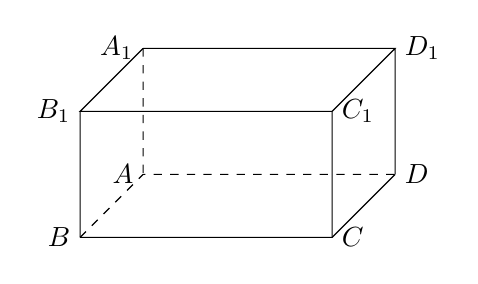
\begin{tikzpicture}[scale=0.8] 
		\coordinate (A) at (0,0)   node at (A) [left] {$A$};
		\coordinate (B) at (-1,-1) node at (B) [left] {$B$};
		\coordinate (C) at (3,-1)  node at (C) [right] {$C$};
		\coordinate (D) at (4,0)   node at (D) [right] {$D$};
		\coordinate (A_1) at (0,2)   node at (A_1) [left] {$A_1$};
		\coordinate (B_1) at (-1,1) node at (B_1) [left] {$B_1$};
		\coordinate (C_1) at (3,1)  node at (C_1) [right] {$C_1$};
		\coordinate (D_1) at (4,2)   node at (D_1) [right] {$D_1$};
		\draw [dashed] (B)--(A)--(D) (A_1)--(A);
		\draw (A_1)--(B_1)--(C_1)--(D_1)--(A_1) (B_1)--(B) (C_1)--(C) (D_1)--(D);
		\draw (B)--(C)--(D);
\end{tikzpicture}}
	\loigiai{ 
		$\overrightarrow{AA_1}+\overrightarrow{AB}+\overrightarrow{AD}=\overrightarrow{AC_1}$ là khẳng định đúng. 
}\end{ex}
\cham{1}
\begin{ex}
	\immini[thm]{Cho hình hộp ${ABCD.EFGH}$. Tìm khẳng định đúng. 
	\choice
	{ $\overrightarrow{AE}+\overrightarrow{AB}+\overrightarrow{AD}=\overrightarrow{CE}$ }
	{ \True $\overrightarrow{AE}+\overrightarrow{AB}+\overrightarrow{AD}=\overrightarrow{AG}$ }
	{ $\overrightarrow{AE}+\overrightarrow{AB}+\overrightarrow{AD}=\overrightarrow{GE}$ }
	{ $\overrightarrow{AE}+\overrightarrow{AB}+\overrightarrow{AD}=\overrightarrow{EG}$ }
}{
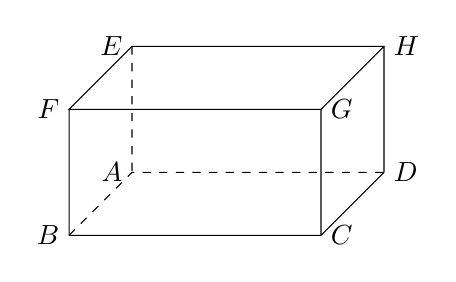
\begin{tikzpicture}[scale=0.8] 
		\coordinate (A) at (0,0)   node at (A) [left] {$A$};
		\coordinate (B) at (-1,-1) node at (B) [left] {$B$};
		\coordinate (C) at (3,-1)  node at (C) [right] {$C$};
		\coordinate (D) at (4,0)   node at (D) [right] {$D$};
		\coordinate (E) at (0,2)   node at (E) [left] {$E$};
		\coordinate (F) at (-1,1) node at (F) [left] {$F$};
		\coordinate (G) at (3,1)  node at (G) [right] {$G$};
		\coordinate (H) at (4,2)   node at (H) [right] {$H$};
		\draw [dashed] (B)--(A)--(D) (E)--(A);
		\draw (E)--(F)--(G)--(H)--(E) (F)--(B) (G)--(C) (H)--(D);
		\draw (B)--(C)--(D);
\end{tikzpicture}}
	\loigiai{ 
		$\overrightarrow{AE}+\overrightarrow{AB}+\overrightarrow{AD}=\overrightarrow{AG}$ là khẳng định đúng. 
}\end{ex}
\cham{1}

\begin{ex}%[1H3B1-2]
	\immini[thm]{Cho hình hộp $ABCD.A'B'C'D'.$ Trong các khẳng định sau, khẳng định nào \textbf{sai}?
		\choice
		{$\vec{AB}+\vec{B'D'}=\vec{AD}$}
		{$\vec{AB}+\vec{CD}=\vec{0}$}
		{$\vec{AC'}+\vec{A'C}=2\vec{AC}$}
		{\True $\vec{AC}-\vec{D'D}=\vec{0}$}}{
		\begin{tikzpicture}[scale=0.55, font=\footnotesize, line join=round, line cap=round]
			\foreach \x\y\t in {0/0/A,-2/-1.5/B,3.9/0/D,-0.5/3.5/A'}
			\coordinate (\t) at (\x,\y);
			\coordinate (C) at ($(B)+(D)-(A)$);
			\coordinate (B') at ($(A')+(B)-(A)$);
			\coordinate (C') at ($(B')+(C)-(B)$);
			\coordinate (D') at ($(C')+(D)-(C)$);
			\draw (A')--(B')--(B)--(C)--(C');
			\draw (A')--(D')--(D);
			\draw (D')--(C') (C)--(D);
			\draw (B')--(C') (D)--(D');
			\draw[dashed] (A)--(B) (A')--(A)--(D);
			\foreach \t/\g in {A/180,B/180,C/0,D/0,A'/180,B'/180,C'/0,D'/0} \draw (\t) node[shift={(\g:10pt)}]{$\t$};
	\end{tikzpicture}}
	\loigiai{
		\immini{
			\begin{itemize}
				\item [$\bullet$] $\vec{AB}+\vec{B'D'}=\vec{AB}+\vec{BD}=\vec{AD}$'
				\item [$\bullet$] $\vec{AB}$ và $\vec{CD}$ đối nhau nên $\vec{AB}+\vec{CD}=\vec{0}$.
				\item [$\bullet$] Theo quy tắc hình bình hành ta có\\ $\vec{AC'}+\vec{A'C}=\vec{AC}+\vec{AA'}+\vec{A'A}+\vec{A'C'}=2\cdot\vec{AC}.$
				\item [$\bullet$] $\vec{AC}-\vec{D'D}=\vec{AC}+\vec{CC'}=\vec{AC'}$
			\end{itemize}
		}
		{\begin{tikzpicture}[scale=0.55, font=\footnotesize, line join=round, line cap=round]
				\foreach \x\y\t in {0/0/A,-2/-1.5/B,3.9/0/D,-0.5/3.5/A'}
				\coordinate (\t) at (\x,\y);
				\coordinate (C) at ($(B)+(D)-(A)$);
				\coordinate (B') at ($(A')+(B)-(A)$);
				\coordinate (C') at ($(B')+(C)-(B)$);
				\coordinate (D') at ($(C')+(D)-(C)$);
				\draw (A')--(B')--(B)--(C)--(C');
				\draw (A')--(D')--(D);
				\draw (D')--(C') (C)--(D);
				\draw (B')--(C') (D)--(D');
				\draw[dashed] (A)--(B) (A')--(A)--(D) (A)--(C') (A')--(C);
				\foreach \t/\g in {A/180,B/180,C/0,D/0,A'/180,B'/180,C'/0,D'/0} \draw (\t) node[shift={(\g:10pt)}]{$\t$};
		\end{tikzpicture}}
		
	}
\end{ex} \cham{2}
\begin{ex}%Câu 6
	\immini[thm]{
		(TN.2025) Cho hình lăng trụ $ABC.A'B'C'$ (xem hình dưới). Phát biểu nào sau đây là \textbf{đúng}?
		\choice
		{$\overrightarrow{BA}+\overrightarrow{A'C'}=\overrightarrow{A'A}$}
		{\True $\overrightarrow{BA}+\overrightarrow{A'C'}=\overrightarrow{BC}$}
		{$\overrightarrow{BA}+\overrightarrow{A'C'}=\overrightarrow{BC'}$}
		{$\overrightarrow{BA}+\overrightarrow{A'C'}=\overrightarrow{C'B'}$}
	}{
	\begin{tikzpicture}[scale=0.8, font=\footnotesize,>=stealth]
		\path
		(0,0) coordinate (A)
		(4,0) coordinate (C)
		(1.5,-1.5) coordinate (B)
		($(A)+(0.4,3)$)coordinate (A')
		($(B)+(0.4,3)$)coordinate (B')
		($(C)+(0.4,3)$)coordinate (C')
		;
		\draw (B)--(C)--(C')--(B')--(B)--(A)--(A')--(B') (A')--(C');
		\draw[dashed] (A)--(C);
		\foreach \x/\g in {A/180,B/-45,C/0,A'/180,B'/190,C'/0}\draw[fill=black] (\x) circle (.04) +(\g:.4)node{\footnotesize$\x$};
	\end{tikzpicture}
	}
	\loigiai{
		$\overrightarrow{BA}+\overrightarrow{A'C'}=\overrightarrow{BA}+\overrightarrow{AC}=\overrightarrow{BC}$.
	}
\end{ex}
\cham{2}
\begin{ex} % Câu 8
	\immini[thm]{(TN.2025) Cho hình chóp tứ giác đều $S.ABCD$ (xem hình bên). Gọi $O$ là giao điểm của $AC$ và $BD$. Phát biểu nào sau đây là đúng?
		\choice
		{$\overrightarrow {SA}  + \overrightarrow {SB}  + \overrightarrow {SC}  + \overrightarrow {SD}  = 2\overrightarrow {SO} $}
		{\True $\overrightarrow {SA}  + \overrightarrow {SB}  + \overrightarrow {SC}  + \overrightarrow {SD}  = 4\overrightarrow {SO} $}
		{$\overrightarrow {SA}  + \overrightarrow {SB}  + \overrightarrow {SC}  + \overrightarrow {SD}  = \overrightarrow {SO} $}
		{$\overrightarrow {SA}  + \overrightarrow {SB}  + \overrightarrow {SC}  + \overrightarrow {SD}  = \overrightarrow 0 $}}
	{\begin{tikzpicture}[scale=0.7, font=\footnotesize,line join=round, line cap=round, >=stealth]
			\coordinate (A) at (0,0);
			\coordinate (B) at (-2.6,-2);
			\coordinate (D) at (5,0);
			\coordinate (C) at ($(B)+(D)-(A)$);
			\coordinate (O) at ($(A)!0.5!(C)$);
			\coordinate (S) at ($(O)+(0,3)$);
			\draw(S)--(B) (S)--(C) (S)--(D) (B)--(C)--(D);
			\draw[dashed,thin](S)--(A)--(C) (A)--(B) (A)--(D)--(B) (S)--(O);
			\foreach \i/\g in {S/90,A/-90,B/-90,C/-90,D/-90,O/-90}{\draw[fill=black](\i) circle (1.5pt) ($(\i)+(\g:4mm)$) node[scale=1]{$\i$};}
	\end{tikzpicture}}
	\loigiai{Ta có: $\overrightarrow {SA}  + \overrightarrow {SB}  + \overrightarrow {SC}  + \overrightarrow {SD}  = \left( {\overrightarrow {SA}  + \overrightarrow {SC} } \right) + \left( {\overrightarrow {SB}  + \overrightarrow {SD} } \right) = 4\overrightarrow {SO} $}
\end{ex}
\cham{3}
\begin{ex}%[Trần Toàn]%[1H3Y1-2]%
	\immini[thm]{Cho tứ diện $ABCD$. Mệnh đề nào dưới đây là mệnh đề đúng?
		\choice
		{$\vec {AB}-\vec {AD}=\vec {CD}+\vec {BC}$}
		{$\vec {AC}-\vec {AD}=\vec {BD}-\vec {BC}$}
		{$\vec {BC}+\vec {AB}=\vec {DA}-\vec {DC}$}
		{\True $\vec {AB}-\vec {AC}=\vec {DB}-\vec {DC}$}}{
		\begin{tikzpicture}[scale=0.8, font=\footnotesize,>=stealth]
			\path
			(0,0) coordinate (A)
			(5,0) coordinate (C)
			(1.2,-1.5) coordinate (B)
			($(B)!0.5!(C)$)coordinate (M)
			($(A)!2/3!(M)$)coordinate (G)
			($(G)+(0,3)$)coordinate (D)
			;
			\draw (D)--(A)--(B)--(D)--(C)--(B);
			\draw[dashed] (A)--(C);
			\foreach \x/\g in {A/180,B/-90,C/0,D/90}\draw[fill=black] (\x) circle (.04) +(\g:.4)node{\footnotesize$\x$};
	\end{tikzpicture}}
	\loigiai{
		Ta có $\vec{AB}-\vec{AC}=\vec{CB}=\vec{DB}-\vec{DC}$.
	}
\end{ex} \cham{4}

\begin{ex}%[1H3B1-2]%
	\immini[thm]{Cho tứ diện $ABCD$. Gọi $ G$ là trọng tâm tam giác $ABC$. Tìm $ k$ thỏa đẳng thức vectơ $\vec{DA}+\vec{DB}+\vec{DC}=k\cdot\vec{DG}$.
		\haicot
		{$ k=1$}
		{$ k=\dfrac{1}{2}$}
		{$ k=2$}
		{\True $ k=3$}}{
		\begin{tikzpicture}[scale=0.8, font=\footnotesize,>=stealth]
			\path
			(0,0) coordinate (A)
			(5,0) coordinate (C)
			(1.2,-1.5) coordinate (B)
			($(B)!0.5!(C)$)coordinate (M)
			($(A)!2/3!(M)$)coordinate (G)
			($(G)+(0,3)$)coordinate (D)
			;
			\draw (D)--(A)--(B)--(D)--(C)--(B);
			\draw[dashed] (A)--(C) (D)--(G);
			\foreach \x/\g in {A/180,B/-90,C/0,D/90,G/0}\draw[fill=black] (\x) circle (.04) +(\g:.4)node{\footnotesize$\x$};
	\end{tikzpicture}}
	\loigiai{
		\immini{
			$\vec{DA}+\vec{DB}+\vec{DC}=\vec{DG}+\vec{GA}+\vec{DG}+\vec{GB}+\vec{DG}+\vec{GC}=3\vec{DG}$.}
		{\begin{tikzpicture}[scale=1, font=\footnotesize,>=stealth]
				\path
				(0,0) coordinate (A)
				(4,0) coordinate (C)
				(1.5,-1.5) coordinate (B)
				($(B)!0.5!(C)$)coordinate (M)
				($(A)!2/3!(M)$)coordinate (G)
				($(G)+(0,3)$)coordinate (D)
				;
				\draw (D)--(A)--(B)--(D)--(C)--(B);
				\draw[dashed] (A)--(C) (D)--(G) (B)--(G)--(A) (G)--(C);
				\foreach \x/\g in {A/180,B/-90,C/0,D/90,G/0}\draw[fill=black] (\x) circle (.04) +(\g:.4)node{\footnotesize$\x$};
			\end{tikzpicture}
		}
	}
\end{ex} \cham{4}

\begin{ex}%[1H3B1-3]
	\immini[thm]{Cho hình lăng trụ $ABC.A'B'C'$. Gọi $G'$ là trọng tâm của tam giác $A'B'C'$. Đặt $\vec{a}=\vec{AA'}, \vec{b}=\vec{AB}, \vec{c}=\vec{AC}$. Véc-tơ $\vec{AG'}$ bằng
		\choice
		{$\dfrac{1}{3}\left(\vec{a}+3\vec{b}+\vec{c}\right)$}
		{\True $\dfrac{1}{3}\left(3\vec{a}+\vec{b}+\vec{c}\right)$}
		{$\dfrac{1}{3}\left(\vec{a}+\vec{b}+3\vec{c}\right)$}
		{$\dfrac{1}{3}\left(\vec{a}+\vec{b}+\vec{c}\right)$}}{
		\begin{tikzpicture}[scale=0.8, font=\footnotesize,>=stealth]
			\path
			(0,0) coordinate (A)
			(4,0) coordinate (C)
			(1.5,-1.5) coordinate (B)
			($(A)+(0.4,3)$)coordinate (A')
			($(B)+(0.4,3)$)coordinate (B')
			($(C)+(0.4,3)$)coordinate (C')
			($(B')!0.5!(C')$)coordinate (I)
			($(A')!2/3!(I)$)coordinate (G')
			;
			\draw (B)--(C)--(C')--(B')--(B)--(A)--(A')--(B') (I)--(A')--(C');
			\draw[dashed] (A)--(C);
			\foreach \x/\g in {A/180,B/-45,C/0,A'/180,B'/190,C'/0,G'/-90}\draw[fill=black] (\x) circle (.04) +(\g:.4)node{\footnotesize$\x$};
	\end{tikzpicture}}
	\loigiai{\vspace{-0.5cm}
		\immini{
			Gọi $I$ là trung điểm của $B'C'$. \\
			Vì $G'$ là trọng tâm của tam giác $A'B'C' \Rightarrow \vec{A'G'}=\dfrac{2}{3}\vec{A'I}$. \\
			$\begin{aligned}
				\text{Ta có } \vec{AG'}&=\vec{AA'}+\vec{A'G'}=\vec{AA'}+\dfrac{2}{3}\vec{A'I}\\
				&=\vec{AA'}+\dfrac{1}{3}\left(\vec{A'B'}+\vec{A'C'}\right)\\
				&=\vec{AA'}+\dfrac{1}{3}\left(\vec{AB}+\vec{AC}\right)\\
				&=\dfrac{1}{3}\left(3\vec{AA'}+\vec{AB}+\vec{AC}\right)=\dfrac{1}{3}\left(3\vec{a}+\vec{b}+\vec{c}\right).
			\end{aligned}$}
		{\begin{tikzpicture}[scale=0.7, font=\footnotesize,>=stealth]
				\path
				(0,0) coordinate (A)
				(4,0) coordinate (C)
				(1.5,-1.5) coordinate (B)
				($(A)+(0.4,3)$)coordinate (A')
				($(B)+(0.4,3)$)coordinate (B')
				($(C)+(0.4,3)$)coordinate (C')
				($(B')!0.5!(C')$)coordinate (I)
				($(A')!2/3!(I)$)coordinate (G')
				;
				\draw (B)--(C)--(C')--(B')--(B)--(A)--(A')--(B') (I)--(A')--(C');
				\draw[dashed] (A)--(C);
				\foreach \x/\g in {A/180,B/-45,C/0,A'/180,B'/190,C'/0,G'/-90,I/-90}\draw[fill=black] (\x) circle (.04) +(\g:.4)node{\footnotesize$\x$};
	\end{tikzpicture}}}
\end{ex} \cham{5}

\begin{ex} 
	\immini[thm]{Cho hình lập phương $ ABCD.A'B'C'D'$ cạnh $ a$. Khẳng định nào sau đây là khẳng định \textbf{sai}?
		\choice
		{$\big|\vec{AC}\big|=a\sqrt{2}$}
		{$\big|\vec{AC'}\big|=a\sqrt{3}$}
		{$\vec{BD}+\vec{D'B'}=\vec{0}$}
		{\True $\vec{BA}+\vec{BC}+\vec{BB'}=\vec{BC'}$}
	}{
		\begin{tikzpicture}[scale=0.55, font=\footnotesize, line join=round, line cap=round]
			\foreach \x\y\t in {0/0/A,-2/-1.5/B,3.9/0/D,0/3.5/A'}
			\coordinate (\t) at (\x,\y);
			\coordinate (C) at ($(B)+(D)-(A)$);
			\coordinate (B') at ($(A')+(B)-(A)$);
			\coordinate (C') at ($(B')+(C)-(B)$);
			\coordinate (D') at ($(C')+(D)-(C)$);
			\draw (A')--(B')--(B)--(C)--(C');
			\draw (A')--(D')--(D);
			\draw (D')--(C') (C)--(D);
			\draw (B')--(C') (D)--(D');
			\draw[dashed] (A)--(B) (A')--(A)--(D) (C)--(A)--(C');
			\foreach \t/\g in {A/180,B/180,C/0,D/0,A'/180,B'/180,C'/0,D'/0} \draw (\t) node[shift={(\g:10pt)}]{$\t$};
		\end{tikzpicture}
	}
	\loigiai{
	}
\end{ex} \cham{9}


\begin{ex}%[1H3B1-2]%
	Cho hình lập phương $ ABCD.A'B'C'D'$ cạnh $ a$. Tính độ dài vectơ $\vec x=\vec{AB'}+\vec{AD'}$ theo $ a$.
	\choice
	{$\left|\vec x\right|=a\sqrt 2 $}
	{$\left|\vec x\right|=2a\sqrt 2 $}
	{$\left|\vec x\right|=2a\sqrt 6 $}
	{\True $\left|\vec x\right|=a\sqrt 6 $}
	\loigiai{
		\immini{Ta có $\vec x=\vec{AB'}+\vec{AD'}=2\vec{AI}$, với $ I$ là trung điểm của $ B'D'$. Khi đó $\left|\vec x\right|=2AI$.\\
			Do tam giác $ AB'D'$ đều cạnh $ a\sqrt 2 $ nên $ AI=\dfrac{a\sqrt 6}{2}$. \\
			Vậy $\left|\vec x\right|=a\sqrt 6 $.}
		{\begin{tikzpicture}[scale=1, font=\footnotesize, line join=round, line cap=round, >=stealth]
				\def\bc{4} % cạnh BC
				\def\ba{2} % cạnh BA
				\def\gocB{35} % góc B của đáy
				\coordinate[label=below left:$B$] (B) at (0,0);
				\coordinate[label=above left:$A$] (A) at (\gocB:\ba);
				\coordinate[label=below:$C$] (C) at (\bc,0);
				\coordinate[label=right:$D$] (D) at ($(C)-(B)+(A)$);
				\coordinate[label=above left:$A'$] (A') at ($(A)+(90:\bc)$);
				\coordinate[label=left:$B'$] (B') at ($(B)-(A)+(A')$);
				\coordinate[label=below right:$C'$] (C') at ($(C)-(A)+(A')$);
				\coordinate[label=right:$D'$] (D') at ($(D)-(A)+(A')$);
				\tkzDefMidPoint(B',D') \tkzGetPoint{I}
				\tkzLabelPoints[above](I);
				\draw (B')--(B)--(C)--(D)--(D')--(A')--(B')--(C')--(D') (C)--(C') (B')--(D');
				\draw[dashed] (A')--(A)--(D) (A)--(B) (A)--(B') (A)--(D') (A)--(I);
				\foreach \diem in {A,B,C,D,A',B',C',D',I}\fill (\diem)circle(1.5pt);
		\end{tikzpicture}}
	}
\end{ex} \cham{8}

\begin{ex}%[1H3B1-3]
	\immini[thm]{Hình lập phương $ABCD.A'B'C'D'$ cạnh $a$. Tính độ dài véctơ $\vec{x}=\vec{AA'}+\vec{AC'}$ theo~$a$.
		\haicot
		{$a\sqrt{2}$}
		{$\left(1+\sqrt{3}\right)a$}
		{\True $a\sqrt{6}$}
		{$\dfrac{a\sqrt{6}}{2}$}}{\hspace{1cm}
		\begin{tikzpicture}[scale=0.7, line join=round, line cap=round]
			\tikzset{label style/.style={font=\footnotesize}}
			\tkzDefPoints{0/0/A,-1.3/-1.1/B,2/-1.1/C}
			\coordinate (D) at ($(A)+(C)-(B)$);
			\coordinate (A') at ($(A)+(0,2.5)$);
			\tkzDefPointsBy[translation=from A to A'](B,C,D){B'}{C'}{D'}
			\tkzDrawPolygon(A',B',B,C,D,D')
			\tkzDrawSegments(B',C' C',D' C,C')
			\tkzDrawSegments[dashed](A,B A,D A,A')
			\tkzDrawPoints[fill=black,size=4](A,B,D,C,A',B',C',D')
			\tkzLabelPoints[above](A',D')
			\tkzLabelPoints[below](A,B,C)
			\tkzLabelPoints[left](B')
			\tkzLabelPoints[right](C',D)
	\end{tikzpicture}}
	\loigiai{
		\immini{
			Gọi $O'$ là tâm $A'B'C'D'\Rightarrow A'O'=\dfrac{a\sqrt{2}}{2}$.\\
			Ta có $\vec{AA'}+\vec{AC'}=2\vec{AO'}\Rightarrow \vert \vec{x} \vert =2\left| \vec{AO'} \right| =2AO'$.\\
			$\triangle AA'O'$ vuông tại $A'\Rightarrow AO'=\sqrt{AA'^2+A'O'^2}=\dfrac{a\sqrt{6}}{2}$.\\
			Vậy $\vert \vec{x} \vert =2AO'=a\sqrt{6}$.
		}{
			\begin{tikzpicture}[scale=.5, line join=round, line cap=round,>=stealth]
				\tkzDefPoints{0/0/B,3/2/A,10/2/D,7/0/C,0/7/B',3/9/A',7/7/C',10/9/D'}
				\tkzInterLL(A',C')(B',D')\tkzGetPoint{O'}
				\tkzDrawSegments[](A',B' B',C' C',D' D',A' B,C C,D B,B' C,C' D,D' A',C' B',D')
				\tkzDrawSegments[dashed](A,A' A,B A,D A,C' A,O')
				\tkzLabelPoints[above](A',D',O')
				\tkzLabelPoints[above left](A,B')
				\tkzLabelPoints[below left](B)
				\tkzLabelPoints[below right](C,C')
				\tkzLabelPoints[right](D)
				\tkzDrawPoints[fill=black](A,B,C,D,A',B',C',D',O')
			\end{tikzpicture}
		}
	}
\end{ex} \cham{8}

\begin{ex}%[2H2H1-4]
	\immini[thm]{
		Trong điện trường đều, lực tĩnh điện $\vec{F}$ (đơn vị: N) tác dụng lên điện tích điểm có điện tích $q$ (đơn vị: C) được tính theo công thức $\vec{F}=q \cdot \vec{E}$, trong đó $\vec{E}$ là cường độ điện trường (đơn vị: N/C). Tính độ lớn của lực tĩnh điện tác dụng lên điện tích điểm khi $q=10^{-9}$ C và độ lớn điện trường $E=10^5$ N/C.
		\choice
		{$10^{-3}$ N}
		{$10^{4}$ N}
		{$10^{-14}$ N}
		{\True $10^{-4}$ N}
		
	}{\hspace{1cm}
		\begin{tikzpicture}[scale=.7]
			\def\drong{3} %  khoảng cách giữa 2 thanh
			\def\drog{0.3} % một nữa độ rộng của thanh
			\def\num{8}
			\filldraw [green!5, draw=green!80!black] ($(0,0)+(-\drog,\drog)$) rectangle ($(0,0)+(\num,0)+(\drog,-\drog)$)
			($(0,-\drong)+(-\drog,\drog)$) rectangle ($(0,-\drong)+(\num,0)+(\drog,-\drog)$); 
			\foreach \a in {0,1,...,\num}{
				\draw[->,>=Latex] ($(0,0)+(\a,0)$)node[red]{$+$}  ($(0,0)+(\a,0)+(0,-\drog)$)-- ($(0,-0.5*\drong)+(\a,0)$);
				\draw ($(0,-0.5*\drong)+(\a,0)$) -- ($(0,-\drong)+(\a,0)+(0,\drog)$) ($(0,-\drong)+(\a,0)$)node[red]{$-$} ;}
			\draw[->,>=Latex] (3.5,-0.4*\drong)--++(-90:1)node[below]{$\vec{F}$};
			\filldraw [green!5, draw=green!80!black]  (3.5,-0.4*\drong)node[green!90!black]{$+$} circle (0.2cm) ;
			\draw (4.5,-0.5*\drong)node{$M$} (8.5,-0.5*\drong)node[red]{$\vec{E}$};
		\end{tikzpicture}
	}
	\loigiai{
		Từ công thức $\vec{F}=q \cdot \vec{E}$ suy ra $\begin{aligned}[t]
			|\vec{F}|	&=q|\vec{E}| \\
			&=10^{-9} \cdot 10^5\\
			&=10^{-4} \text{ N}.
		\end{aligned}$\\
		Vậy độ lớn của lực tĩnh điện tác dụng lên điện tích điểm là $10^{-4}$ N.
	}
\end{ex} \cham{4}

\begin{ex} 
	\immini[thm]{
		Một chiếc đèn tròn được treo song song với mặt phẳng nằm ngang bởi ba sợi dây không dãn xuất phát từ điểm $O$ trên trần nhà và lần lượt buộc vào ba điểm $A$, $B$, $C$ trên đèn tròn sao cho các lực căng $\vec{F_1}$, $\vec{F_2}$, $\vec{F_3}$ lần lượt trên mỗi dây $OA$, $OB$, $OC$ đôi một vuông góc với nhau và $\left| \vec{F_1} \right| = \left| \vec{F_2} \right| = \left| \vec{F_3} \right|$ = $15$ (N). Tính trọng lượng của chiếc đèn tròn đó.
		\haicot
		{$14\sqrt{3}$ (N)}
		{\True $15\sqrt{3}$ (N)}
		{$17\sqrt{3}$ (N)}
		{$16\sqrt{3}$ (N)}
	}{\hspace{1cm}
		\begin{tikzpicture}[scale=0.6, font=\footnotesize, line
			join=round, line cap=round]
			%Toa do cac diem
			\coordinate (O) at (0,5); 
			\coordinate (A) at (-2.2163, -0.4626);
			\coordinate (C) at (2.5, 0.1);
			\coordinate (B) at (-1.245, 0.867);
			\coordinate (A_1) at ($(O)!1/2!(A)$);
			\coordinate (B_1) at ($(O)!3/4!(B)$);
			\coordinate (C_1) at ($(O)!1/2!(C)$);	
			%Ve hai day
			\draw[fill=blue!30] (0,-0.44) ellipse ({2.5} and {1});
			\draw[fill=blue!30] (0,0) ellipse ({2.5} and {1});
			%Ve cac doan thang
			\draw[line width=3] (-3,5)--(3,5);
			\draw(O)--(A);
			\draw(O)--(B);
			\draw(O)--(C);
			\draw[dashed] (0,0)--(C);
			\draw[dashed] (0,0)--(0,-2.5/2);
			%Ve cac diem
			\draw(A) node[above right]{$A$};
			\draw(B) node[above right]{$B$};
			\draw(C) node[above right]{$C$};
			\draw(C) node[above right]{$C$};
			\draw (0.2,5) node [below right]{$O$};
			\draw [fill=red] (0,0) circle (3.2pt); 
			%Ve cac vecto
			\draw[-stealth, very thick, blue] (O)--(A_1) node [pos=0.5, left]{$\vec{F_1}$};
			\draw[-stealth, very thick, blue] (O)--(B_1) node [pos=0.5, right]{$\vec{F_2}$};
			\draw[-stealth, very thick, blue] (O)--(C_1) node [pos=0.5, right]{$\vec{F_3}$};
			\draw[-stealth,very thick](0,-2.5/2)--(0,-3.5) node [pos=0.5, right]{$\vec{P}$};
	\end{tikzpicture}}
	\loigiai{
		\immini{
			Gọi $A_1$, $B_1$, $C_1$ lần lượt là các điểm sao cho $\vec{OA_1} = \vec{F_1}$, $\vec{OB_1} = \vec{F_2}$, $\vec{OC_1} = \vec{F_3}$. Lấy các điểm $D_1$, $A_1'$, $B_1'$, $D_1'$ sao cho $OA_1D_1B_1.C_1A_1'D_1'B_1'$ là hình hộp (như hình bên). Khi đó, áp dụng quy tắc hình hộp ta có
			$$\vec{OA_1}+\vec{OB_1}+\vec{OC_1}=\vec{OD_1'}.$$
			Mặt khác, do các lực căng $\vec{F_1}$, $\vec{F_2}$, $\vec{F_3}$ đôi một vuông góc và $\left| \vec{F_1} \right| = \left| \vec{F_2} \right| = \left| \vec{F_3} \right|$ = $15$ (N) nên hình hộp $OA_1D_1B_1.C_1A_1'D_1'B_1'$ có ba cạnh $OA_1$, $OB_1$, $OC_1$ đôi một vuông góc và bằng nhau. Vì thế hình hộp đó là hình lập phương có độ dài cạnh bằng $15$. Suy ra độ dài đường chéo $OD_1'$ của hình lập phương đó bằng $15 \sqrt{3}$.\\
			Do chiếc đèn ở vị trí cân bằng nên $\vec{F_1}+\vec{F_2}+\vec{F_3}=\vec{P}$, ở đó $\vec{P}$ là trọng lực tác dụng lên chiếc đèn. Suy ra trọng lượng của chiếc đèn là $\left| \vec{P} \right| = \left| \vec{OD_1'} \right| =15\sqrt{3}$ (N).
		}{\begin{tikzpicture}[scale=0.6, font=\footnotesize, line join=round, line cap=round]
				\foreach \x\y\t in {0/0/B_1,-3.5/-3.5/D_1,2.5/-2.5/B_1',-0.6/3/O}
				\coordinate (\t) at (\x,\y);
				\coordinate (D_1') at ($(B_1')+(D_1)-(B_1)$);
				\coordinate (A_1) at ($(O)+(D_1)-(B_1)$);
				\coordinate (A_1') at ($(A_1)+(D_1')-(D_1)$);
				\coordinate (C_1) at ($(O)+(B_1')-(B_1)$);
				\draw (D_1)--(D_1')--(B_1');
				\draw (D_1)--(A_1)--(A_1')--(D_1');
				\draw (A_1')--(C_1)--(B_1');
				\draw[dashed] (D_1)--(B_1)--(B_1');
				\draw[-stealth] (O)--(A_1)node [pos=0.5, above left]{$\vec{F_1}$};
				\draw[-stealth] (O)--(C_1) node [pos=0.5, above right]{$\vec{F_3}$};
				\draw[dashed, -stealth] (O)--(B_1) node [pos=0.5, right]{$\vec{F_2}$};
				\draw[dashed, -stealth] (O)--(D_1');
				\foreach \t/\g in {B_1/-80,D_1/180,D_1'/-30,B_1'/0,O/100,A_1/180,A_1'/-160,C_1/0} \draw (\t) node[shift={(\g:10pt)}]{$\t$};
		\end{tikzpicture}}
	}
\end{ex} \cham{12}

\begin{ex}%[2H2V1-4]
	\immini[thm]{
		Một chiếc đèn chùm treo có khối lượng $m=5 \mathrm{\,kg}$ được thiết kế với đĩa đèn được giữ bởi bốn đoạn xích $SA$, $SB$, $SC$, $SD$ sao cho $S.ABCD$ là hình chóp tứ giác đều có $\widehat{ASC}=60^{\circ}$. Tìm độ lớn của lực căng cho mỗi sợi xích. Lấy $g=10 \mathrm{\,m/s}^2$.
		\haicot
		{$\dfrac{15\sqrt{3}}{3} \mathrm{\,N}$}
		{$\dfrac{20\sqrt{3}}{3} \mathrm{\,N}$}
		{$\dfrac{25\sqrt{3}}{3} \mathrm{\,N}$}
		{\True $\dfrac{30\sqrt{3}}{3} \mathrm{\,N}$}
	}
	{\includegraphics[width=3.7cm]{Images/den-1.png}}
	\loigiai{
		\begin{listEX}
			\item [$\bullet$] Ta có $\overrightarrow{P}=m\overrightarrow{g}$ nên $\left|\overrightarrow{P}\right|=m\cdot\left|\overrightarrow{g}\right|=5 \cdot 10=50 \mathrm{\,N}$.\\
			Vậy độ lớn của trọng lực $\overrightarrow{P}$ tác động lên chiếc đèn chùm là $50 \mathrm{\,N}$.
			\item[$\bullet$]  Gọi $O$ là trọng tâm của chiếc đèn chùm cũng là chân đường cao hình chóp đều $S.ABCD$.\\
			Vẽ $\overrightarrow{OP}$ biểu diễn trọng lực tác động lên đèn chùm với $$OP \perp (ABCD).$$
			Khi đó lực căng mỗi sợi xích sẽ là $\overrightarrow{AS}$, $\overrightarrow{BS}$, $\overrightarrow{CS}$, $\overrightarrow{DS}$.\\
			Chiếc đèn chùm đứng yên nên 
			$\overrightarrow{AS}+\overrightarrow{BS}+\overrightarrow{CS}+\overrightarrow{DS}+\overrightarrow{OP}=\overrightarrow{0}$.
			\immini{
				Suy ra $\begin{aligned}[t]
					\overrightarrow{OP}
					&=\overrightarrow{SA}+\overrightarrow{SC}+\overrightarrow{SB}+\overrightarrow{SD}\\
					&=2\overrightarrow{SO}+2\overrightarrow{SO}=4\overrightarrow{SO}.
				\end{aligned}$\\
				Suy ra $SO=\dfrac{1}{4}\cdot OP=\dfrac{50}{4}=\dfrac{25}{2}$.\\
				Tam giác $SAC$ cân tại $S$ có $\cos\widehat{OSA}=\dfrac{SO}{SA}$.\\
				Suy ra lực căng mỗi sợi xích là $SA=\dfrac{SO}{\cos 30^{\circ}}=\dfrac{\tfrac{25}{2}}{\tfrac{\sqrt{3}}{2}}=\dfrac{25\sqrt{3}}{3} \mathrm{\,N}$.
			}{
				\begin{tikzpicture}[scale=0.7, font=\footnotesize, line join=round, line cap=round]
					\foreach \x\y\t in {0/0/A,-1.9/-1./B,1.6/-1./C}
					\coordinate (\t) at (\x,\y);
					\coordinate (D) at ($(A)+(C)-(B)$);
					\coordinate (O) at ($(A)!1/2!(C)$);
					\coordinate (S) at ($(O)+(0,3.)$);
					\coordinate (P) at ($(O)-(0,3.9)$);
					\foreach \a\b in {O/P, B/S,C/S,D/S}
					\draw[-{Stealth[length=1mm]}] (\a)--(\b);
					\draw (S)--(C)--(B)--(S)--(D)--(C);
					\draw[dashed](C)--(A)--(B)--(D)--(A)--(S)--(O);
					\foreach \t/\g in {S/90,A/160,B/-135,C/-70,D/0,O/-135,P/0}
					\draw[fill=black] (\t) circle(1pt)
					node[shift={(\g:7pt)}]{$\t$};
			\end{tikzpicture}}
		\end{listEX}
	}
\end{ex} \cham{12}

\Closesolutionfile{ans}

\ind{PHẦN II.} \inden{Câu trắc nghiệm đúng sai. Trong mỗi ý a), b), c), d) ở mỗi câu, học sinh chọn đúng hoặc sai.}\\
\Opensolutionfile{ans}[ans/2H2-B1-d1-2]
\begin{ex}
	\immini{Cho hình hộp chữ nhật $ABCD.A'B'C'D'$ có cạnh $AB=a$; $AD=a\sqrt{3}$; $AA'=2a$. Xét tính đúng, sai của các khẳng định sau:
		\choiceTF
		{$\vec{AB'}+\vec{CD'}=\vec{0}$}
		{\True $\vec{A'D}+\vec{CB'}=\vec{0}$}
		{$\big|\vec{AB}+\vec{AD}\big|=a\sqrt{5}$}
		{\True $\big|\vec{AB}+\vec{A'D'}+\vec{CC'}\big|=2\sqrt{2}a$}}{
		\begin{tikzpicture}[scale=0.7, font=\footnotesize, line join=round, line cap=round]
			\def\h{4}
			\foreach \x\y\t in {0/0/A,-1/-1.1/B,4.6/-1.1/C}
			\coordinate (\t) at (\x,\y);
			\coordinate (D) at ($(A)+(C)-(B)$);
			\coordinate (A') at ($(A)+(0,3.2)$);
			\coordinate (B') at ($(B)+(0,3.2)$);
			\coordinate (C') at ($(C)+(0,3.2)$);
			\coordinate (D') at ($(D)+(0,3.2)$);
			\draw (B')--(A')--(D')--(C')--(B')--(B)--(C)--(D)--(D') (C')--(C);
			\draw[dashed](B)--(A)--(D) (A)--(A');
			\foreach \t/\g in {A/170,B/-150,C/-70,D/0,A'/100,B'/170,C'/-20,D'/50}
			\draw[fill=black] (\t) circle(1pt)
			node[shift={(\g:7pt)}]{$\t$};
	\end{tikzpicture}}
	\loigiai{\begin{enumerate}[a)]
			\item $\vec{AB'}$ và $\vec{CD'}$ không đối nhau nên $\vec{AB'}+\vec{CD'} \ne \vec{0}$
			\item $\vec{A'D}$ và $\vec{CB'}$ đối nhau nên $\vec{AB'}+\vec{CD'} = \vec{0}$
			\item $\big|\vec{AB}+\vec{AD}\big|=\big|\vec{AC}\big|=AC=\sqrt{AB^2+AD^2}=2a$
			\item $\big|\vec{AB}+\vec{A'D'}+\vec{CC'}\big|=\big|\vec{AB}+\vec{AD}+\vec{AA'}\big|=AC'=\sqrt{AB^2+AD^2+AA^2}=2\sqrt{2}a$
	\end{enumerate}}
\end{ex} \cham{10}

\begin{ex}%[2H2H1-2]
	\immini{Cho hình lập phương $ABCD.A'B'C'D'$ có cạnh bằng $a$. Xét tính đúng, sai của các khẳng định sau:
		\choiceTF
		{\True $\vec{B'B} - \vec{DB} = \vec{B'D}$}
		{$\vec{BA}+\vec{BC}+\vec{BB'}=\vec{BD}$}
		{$\big|\vec{BA}+\vec{BC}+\vec{BB'}\big|=a\sqrt{2}$}
		{\True $\big|\vec{BC}-\vec{BA}+\vec{C'A}\big|=a$}
	}{
		\begin{tikzpicture}[scale=0.7, font=\footnotesize, line join=round, line cap=round]
			\def\h{4}
			\foreach \x\y\t in {0/0/A,-1/-1.1/B,2.6/-1.1/C}
			\coordinate (\t) at (\x,\y);
			\coordinate (D) at ($(A)+(C)-(B)$);
			\coordinate (A') at ($(A)+(0,3.2)$);
			\coordinate (B') at ($(B)+(0,3.2)$);
			\coordinate (C') at ($(C)+(0,3.2)$);
			\coordinate (D') at ($(D)+(0,3.2)$);
			\draw (B')--(A')--(D')--(C')--(B')--(B)--(C)--(D)--(D') (C')--(C);
			\draw[dashed](B)--(A)--(D) (A)--(A');
			\foreach \t/\g in {A/170,B/-150,C/-70,D/0,A'/100,B'/170,C'/-20,D'/50}
			\draw[fill=black] (\t) circle(1pt)
			node[shift={(\g:7pt)}]{$\t$};
	\end{tikzpicture}}
	\loigiai{
		\immini{\vspace*{-3mm}
			\begin{listEX}
				\item Ta có \begin{eqnarray*}
					\vec{B'B} - \vec{DB} &=& \vec{B'B} + \left( - \vec{DB} \right) \\
					&=& \vec{B'B} + \vec{BD} \\
					&=& \vec{B'D}.
				\end{eqnarray*}
				\item Áp dụng quy tắc hình hộp ta có $\vec{BA}+\vec{BC}+\vec{BB'}=\vec{BD'}$.\\
				\item $\big|\vec{BA}+\vec{BC}+\vec{BB'}\big|=\big|\vec{BD'}\big|=BD'=a\sqrt{3}$
				\item Ta có $\vec{BC}-\vec{BA}+\vec{C'A}=\vec{AC}+\vec{C'A}=\vec{C'C}$.\\
				Do đó $\big|\vec{BC}-\vec{BA}+\vec{C'A}\big|=C'C=a$
		\end{listEX}}
		{
			\begin{tikzpicture}[scale=0.6, font=\footnotesize, line join=round, line cap=round]
				\def\h{4}
				\foreach \x\y\t in {0/0/A,-1/-1.1/B,2.6/-1.1/C}
				\coordinate (\t) at (\x,\y);
				\coordinate (D) at ($(A)+(C)-(B)$);
				\coordinate (A') at ($(A)+(0,3.2)$);
				\coordinate (B') at ($(B)+(0,3.2)$);
				\coordinate (C') at ($(C)+(0,3.2)$);
				\coordinate (D') at ($(D)+(0,3.2)$);
				\draw (B')--(A')--(D')--(C')--(B')--(B)--(C)--(D)--(D') (C')--(C);
				\draw[dashed](B)--(A)--(D) (A)--(A');
				\foreach \t/\g in {A/170,B/-150,C/-70,D/0,A'/100,B'/170,C'/-20,D'/50}
				\draw[fill=black] (\t) circle(1pt)
				node[shift={(\g:7pt)}]{$\t$};
		\end{tikzpicture}}
	}
\end{ex} \cham{11}

\begin{ex}
	\immini{
		Cho tứ diện $ABCD$. Gọi $M$, $N$ lần lượt là trung điểm của các cạnh $AD$ và $BC$, $I$ là trung điểm $MN$. Xét tính đúng, sai của các khẳng định sau:
		\choiceTF
		{$\vv{A B}-\vv{C D}=\vv{A C}-\vv{B D}$}
		{\True $\vec{AB} + \vec{CD} = \vec{AD} + \vec{CB}$}
		{\True $\vec{AB} + \vec{DC}=2\vec{MN}$}
		{\True $\vec{IA} + \vec{IB} + \vec{IC} + \vec{ID} = \vec{0}$}
	}{
		\vspace*{-3mm}
		\begin{tikzpicture}[scale=0.6, font=\footnotesize, line join=round, line cap=round]
			\foreach \x\y\t in {0/0/B,6/0/D,1.5/-2/C,1.5/5/A}
			\coordinate (\t) at (\x,\y);
			\coordinate (M) at ($(A)!1/2!(D)$);
			\coordinate (N) at ($(B)!1/2!(C)$);
			\coordinate (I) at ($(M)!1/2!(N)$);
			\draw (A)--(B)--(C)--(D)--(A)--(C);
			\draw[dashed] (D)--(I)--(A) (B)--(I)--(C) (M)--(N) (B)--(D);
			\foreach \t/\g in {A/90,B/180,C/-90,D/0,M/0,N/180,I/20} \draw (\t) node[shift={(\g:10pt)}]{$\t$};
	\end{tikzpicture}}	
	\loigiai{
		\begin{enumerate}
			\item  Sử dụng quy tắc ba điểm và quy tắc hiệu, ta có
			\begin{align*}
				\vv{A B}-\vv{C D} &\ =\left(\vv{A C}+\vv{C B}\right)-\vv{C D} \\
				&\ =\vv{A C}+\left(\vv{C B}-\vv{C D}\right) \\
				&\ =\vv{A C}+\vv{D B} \\
				&\ =\vv{A C}-\vv{B D}.
			\end{align*}
			\item  Theo quy tắc ba điểm, ta có $\vec{AB} = \vec{AD} + \vec{DB}$. Do đó
			\begin{eqnarray*}
				\vec{AB} + \vec{CD} &=& \vec{AD} + \vec{DB} + \vec{CD} \\
				&=&\vec{AD}+ \left( \vec{CD} + \vec{DB} \right) \\
				&=& \vec{AD} + \vec{CB}.
			\end{eqnarray*}
			\item Ta có 
			\item 
		\end{enumerate}	
	}
\end{ex} \cham{14} 

\begin{ex}
	\immini
	{
		Một chiếc ô tô được đặt trên mặt đáy dưới của một khung sắt có dạng hình hộp chữ nhật với đáy trên là hình chữ nhật $ABCD$, mặt phẳng $(ABCD)$ song song với mặt phẳng nằm ngang. Khung sắt đó được buộc vào móc $E$ của chiếc cần cẩu sao cho các đoạn dây cáp $EA$, $EB$, $EC$, $ED$ có độ dài bằng nhau và cùng tạo với mặt phẳng $(ABCD)$ một góc bằng $60^\circ$. Chiếc cần cẩu kéo khung sắt lên theo phương thẳng đứng. Biết rằng các lực căng $\vec{F_1}$, $\vec{F_2}$, $\vec{F_3}$, $\vec{F_4}$ đều có cường độ là $4700$ N và trọng lượng của khung sắt là $3000$ N.
		\choiceTF
		{$\vec{F_1}+\vec{F_2}=\vec{F_3}+\vec{F_4}$}
		{\True $\vec{F_1}+\vec{F_3}=\vec{F_2}+\vec{F_4}$}
		{\True $\big|\vec{F_1}+\vec{F_3}\big|=8141$ N (\textit{làm tròn đến hàng đơn vị})}
		{Trọng lượng của chiếc xe ô tô là $16282$ N (\textit{làm tròn đến hàng đơn vị})}
	}
	{\hspace{1cm}
		\includegraphics[scale=.09]{Images/xe-1.jpg}
	}
	\loigiai{
		Lấy các điểm $M$, $N$, $P$, $Q$ lần lượt trên các tia $EA$, $EB$, $EC$, $ED$ sao cho 
		\[
		\vec{EM} = \vec{F_1},\ \vec{EN} = \vec{F_2},\ \vec{EP} = \vec{F_3},\ \vec{EQ} = \vec{F_4}.
		\]
		Do các lực căng $\vec{F_1}$, $\vec{F_2}$, $\vec{F_3}$, $\vec{F_4}$ đều có cường độ là $4700$ N nên $EM = EN = EP = EQ = 4700$.
		\begin{center}
			\begin{tikzpicture}[line join=round, line cap = round, >=stealth, scale=.8,font=\footnotesize,transform shape]
				\foreach \x/\y/\z/\g in
				{
					-3/0/A/180, -1/-1/B/-90, 3/0/C/0, 1/1/D/45, 0/4/E/90
				}
				\draw[fill=black] (\x,\y) circle(1pt) coordinate (\z) ($(\z)+(\g:3.5mm)$) node{$\z$};
				\path
				($(E)!.75!(A)$) coordinate (M)
				($(E)!.75!(B)$) coordinate (N)
				($(E)!.75!(C)$) coordinate (P)
				($(E)!.75!(D)$) coordinate (Q)
				($(M)!.5!(P)$) coordinate (O)
				;
				
				\draw (E)--(A)--(B)--(E)--(C)--(B) (M)--(N)--(P);
				\draw[dashed] (M)--(P)--(Q)--(M) (N)--(Q) (O)--(E)--(D)--(C) (A)--(D);
				
				\foreach \x/\g in {M/135, N/-45,P/45,Q/45,O/135}
				\draw[fill = white] (\x) circle(1pt) ($(\x)+(\g:3mm)$) node{$\x$};
			\end{tikzpicture}
		\end{center}
		\begin{enumerate}[a)]
			\item Ta có
			\begin{itemize}
				\item [$\bullet$] $\vec{F_1}+\vec{F_2}=\vec{EM}+\vec{EN}=2\vec{EH}$, với $H$ là trung điểm của $MN$.
				\item [$\bullet$] $\vec{F_3}+\vec{F_4}=\vec{EP}+\vec{EQ}=2\vec{EK}$, với $K$ là trung điểm của $PQ$.
			\end{itemize}
			Suy ra $\vec{F_1}+\vec{F_2}\ne \vec{F_3}+\vec{F_4}$
			\item Ta có
			\begin{itemize}
				\item [$\bullet$] $\vec{F_1}+\vec{F_3}=\vec{EM}+\vec{EP}=2\vec{EO}$, với $O$ là trung điểm của $MP$.
				\item [$\bullet$] $\vec{F_2}+\vec{F_4}=\vec{EN}+\vec{EQ}=2\vec{EO}$, với $O$ là trung điểm của $MP$.
			\end{itemize}
			Suy ra $\vec{F_1}+\vec{F_3}=\vec{F_2}+\vec{F_4}$.
			\item $\big|\vec{F_1}+\vec{F_3}\big|=\big|2\vec{EO}\big|=2EO$.\\
			Theo giả thiết, góc giữa $EA$ với $(ABCD)$ bằng $60^\circ$, suy ra góc giữa $EM$ với $(MNPQ)$ cũng bằng $60^\circ$ hay $\widehat{SMO}=60^\circ$.\\
			Xét $\triangle EMO$ có $EM=4700$, $\widehat{SMO}=60^\circ$. Suy ra $EO = EM \sin 60^\circ = 2350\sqrt{3}$.\\
			Từ đây, ta tính được $\big|\vec{F_1}+\vec{F_3}\big|=2EO=8141$ N.
			\item Gọi $\vec{P}$ là trọng lực tác dụng lên cả hệ, do $O$ là trung điểm $MP$, $NQ$ nên ta có:
			\begin{eqnarray*}
				& \vec{P} & = \vec{F_1}+\vec{F_2}+\vec{F_3}+\vec{F_4}\\
				& & = \vec{EM } + \vec{EN} + \vec{EP} + \vec{EQ}\\
				& & = \vec{EO} + \vec{OM} + \vec{EO} + \vec{ON} + \vec{EO} + \vec{OP} + \vec{EO} + \vec{OQ}\\
				& & = 4\vec{EO} + \left(\vec{OM} + \vec{OP}\right) + \left(\vec{ON} + \vec{OQ}\right)\\
				& & = 4\vec{EO}. 
			\end{eqnarray*} 
			Suy ra trọng lượng của toàn bộ hệ là $\left| \vec{P} \right| = 4\left| \vec{EO}\right| = 4EO = 9400\sqrt{3}$ N.\\
			Do trọng trượng khung sắt là $3000$ N nên trọng lượng của xe ô tô là $9400\sqrt{3} - 3000 \approx 13281$ N.
		\end{enumerate}
	}
\end{ex} \cham{42}



\Closesolutionfile{ans}